% qjrms4doc.tex V1.10, 4 October 2013

\documentclass[times]{qjrms4}
\usepackage[colorlinks,bookmarksopen,bookmarksnumbered,citecolor=red,urlcolor=red]{hyperref}
\usepackage{moreverb}

%\def\volumeyear{2013}
\def\volumenumber{00}

\begin{document}

\runningheads{A.~R.~Herrington and K.~A.~Reed}{CAM resolution sensitivity}

\title{Parameterized convection, stratiform clouds and resolution sensitivity in the Community Atmosphere Model}

\author{Adam R. Herrington\corrauth \& Kevin A. Reed}
\address{School of Marine and Atmospheric Sciences, Stony Brook University, Stony Brook, NY 11794}

\corraddr{\url{adam.herrington@stonybrook.edu}}

\begin{abstract}
This paper describes...
\end{abstract}

\keywords{Climate models, physical parameterizations, resolution sensitivity}

\maketitle

\section{Introduction}

An increasing number of Atmospheric General Circulation Models (AGCMs) are being developed to maximize efficiency on massively parallel systems, permitting regionally-refined high-resolution, or even globally high-resolution weather ($\Delta x \leq 5$ km) and climate ($\Delta x \leq 50$ km) simulations \citep{SMTMN2008JCP,MPASatm,Z2014QJRMS,HETAL2016JCLIM,DCMIP16,LetAl2018JAMES}. These models are built using unstructured meshes that allows for substantial grid flexibility, but lack physical parameterizations ({\em{physics}}) which behave consistently as the truncation scale of the model changes with different grid resolutions, referred to as scale-aware physics. The most common approach towards developing scale-aware physics is through the lens of limited area, large-eddy simulations \citep[e.g.,][]{PC2008JAS,AW2013JAS,SZ2018JCLIM}. By subsequently filtering large-eddy solutions to lower-resolution grids, a relationship between first- and higher-order moments may be understood and ultimately parameterized as a function of grid resolution. While this approach is likely necessary for developing scale-aware physics, it is not sufficient. The equations of motions have inherent scale dependencies, and the properties of dynamical modes are a function of native grid resolution \citep{O1981JAS,WETAL1997MWR,PG2006JAS,JR2016QJRMS}. Scale-aware physics should also recognize these native grid dependencies.

The sensitivity of the Community Atmosphere Model \citep[CAM;][]{CAM5}, and its predecessor, the Community Climate Model (CCM) to resolution ({\em{resolution}} refers to {\em{horizontal resolution}}, hereafter) is well documented through convergence studies \citep{KW1991JGR,WETAL1995CD,W2008TELLUS,RETAL2013JCLIM,ZetAl2014JCb,HR2017JCLIM}. CAM/CCM is a fully supported, well-funded climate model, but despite thirty years of continual model development, there are robust sensitivities to resolution that have persisted in all versions of the model. This study argues that a unifying cause, the inherent scale sensitivities of the underlying dynamical equations, can explain the robust responses to resolution that occur in CAM/CCM.

In CAM/CCM, the atmosphere progressively dries with increasing resolution, seen through a reduction in simulated total precipitable water \citep{KW1991JGR,WETAL1995CD,W2008TELLUS,RETAL2013JCLIM,ZetAl2014JCb,HR2017JCLIM}, which typically, but not always \citep[see][]{WETAL1995CD,ZetAl2014JCb}, coincides with a reduction in cloud cover. \cite{KW1991JGR} and \cite{WETAL1995CD} suggested that the drying of the atmosphere is due to greater magnitude resolved vertical velocities with increasing resolution, with greater subsiding motion increasing the export of dry air from the upper troposphere. This mechanism is consistent with an analysis of moisture budgets in CAM, version 4 \citep[CAM4;][]{CAM4} across multiple resolutions \citep{YETAL2014JCLIM,HR2017JCLIM}.

It is well known that the magnitude of vertical velocities increase with resolution in atmospheric models. While the cause of this sensitivity has been established for large-eddy simulations \citep[see][and references therein]{J2017JAMES}, only recently has the vertical velocity field in AGCMs and their sensitivity to resolution received attention \citep{DETALA2016ACP,OETAL2016JAMES}, albeit with seemingly conflicting explanations \citep{RETAL2016CD,HR2018JAMES}. To generalize the relationship between vertical velocity and resolution, let $\alpha$ refer to the ratio of $W_0$, the vertical velocity scale of some reference grid spacing $\Delta x_0$, to $W$, the vertical velocity scale for any $\Delta x$. A power law for $\alpha^{-1}$ in $\Delta x$ is then,
\begin{equation}
\alpha^{-1} = \frac{W}{W_0} = \left( \frac{\Delta x}{\Delta x_0} \right)^n, \label{eq:alpha}
\end{equation}
where $n$ is the power law exponent. 

\cite{RETAL2016CD} derive an estimate $n= h-1$ in equation~\ref{eq:alpha} by combining a scale analysis of the continuity equation with a power law representation $\Delta x^{2h}$ of the second-order structure function of the horizontal wind. Strictly speaking, $\Delta x$ here refers to the distance between two points for which the velocity increment is computed in the structure function, but with this distance set to the model grid-spacing. Regional models analyzed in \cite{RETAL2016CD} provide evidence for $h<1$, implying $n<0$ and consistent with the increase in $W$ with resolution in models.

Observations show that $h=\frac{1}{3}$ for horizontal scales on the order of $10^2$ km and less \citep[hereafter referred to as the {\em{mesoscale}};][]{L1999JFM,CL2001JGR}. This value for $h$ is also supported by the slope of the kinetic energy spectrum $-\beta$, which can be related to the second-order structure function through the Weiner–Khinchine theorem, $\beta = \left( 2h+1 \right)$, valid in the range $1<\beta<3$ \citep[satisfies stationarity;][]{DETAL1996JAS}. For $h=\frac{1}{3}$, $\beta=\frac{5}{3}$, which is true for the kinetic energy spectrum in observations \citep{NG1985JAS,CETAL1999JGR} and models \citep[e.g.,][]{THO2006GRL,SPKS2014JAS} at the mesoscale. \cite{RETAL2016CD} propose that the overwhelming support for $h=\frac{1}{3}$ at the mesoscale provides an emergent constraint for $n=-\frac{2}{3}$ in equation~\ref{eq:alpha}.

In large-eddy simulations, the sensitivity of vertical velocities to resolution is adequately explained by a scale analysis of the dynamical equations \citep{WETAL1997MWR,PG2006JAS,JR2016QJRMS}. For hydrostatic scales relevant to AGCMs, a scale analysis of the Poisson equation gives $W \propto D^{-1}$, where $D$ is the horizontal scale of buoyancy perturbations driving vertical motion \citep{HR2018JAMES}. In CAM aqua-planet simulations, the largest source of buoyancy is from stratifrom cloud formation, which are grid-limited with horizontal scales set by the effective resolution of the model \citep[i.e., some multiple of $\Delta x$;][]{S2011LNCSE}, indicating $n=-1$ in equation~\ref{eq:alpha} \citep{HR2018JAMES}. \cite{HR2017JCLIM} has shown that the $n=-1$ scaling does not explain the behavior of CAM4 in a convergence experiment, but follow-up studies \citep{HR2018JAMES,HETAL2019JAMES} indicate that the inadequacy of the $n=-1$ scaling is not definitive, due to large time-truncation errors associated with fixing the physics time-step ($\Delta t_{phys}$) across resolutions in that study.

Another robust response of the CAM/CCM lineage to resolution is an increase in stratiform precipitation rates at the expense of parameterized convective precipitation rates. The resolution dependent partitioning between the two different precipitation routines is shown in Figure~\ref{fig:cam-history}, which is a bar-graph of the climatological, global mean stratiform and convective precipitation rates in prior CAM/CCM convergence studies. The tendency for precipitation rates to shift from the convection scheme to the stratiform scheme with resolution has been documented in other models \citep{PS2002CD,RETAL2016CD,TETAL2018CD}, but none have provided a satisfactory explanation for this sensitivity. The studies of \cite{KW1991JGR}, \cite{WETAL1995CD} and \cite{W2013QJRMS} indicate that the practice of reducing $\Delta t_{phys}$ with resolution should by itself reduce the convective precipitation rates, however Figure~\ref{fig:cam-history} (top row) indicates that convergence studies with fixed $\Delta t_{phys}$ still show a reduction in convective precipitation rates with resolution.

\begin{figure}[t]
\begin{center}
\noindent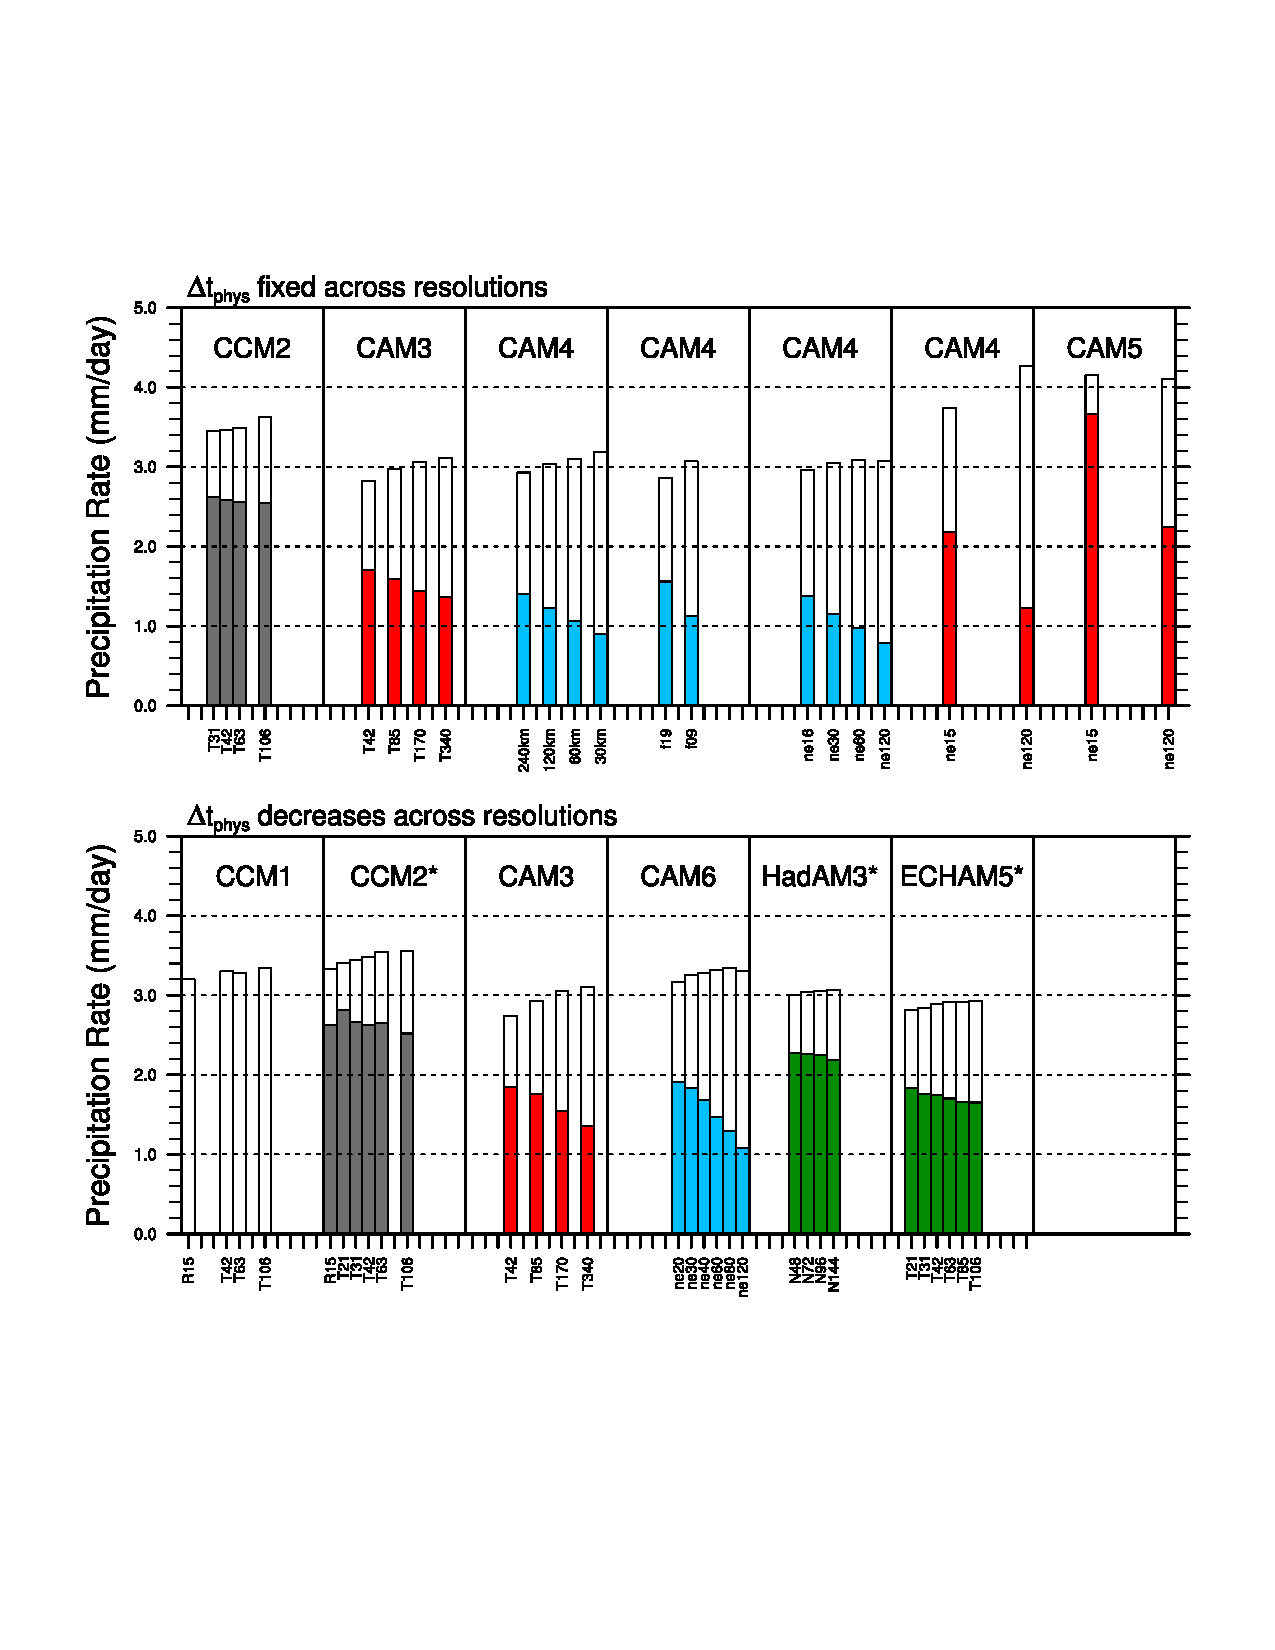
\includegraphics[width=20pc,angle=0]{figs/cam-history.pdf}\\
\end{center}
\caption{Bar-graph of the convective (solid) and stratiform (white) climatological precipitation rates in prior CAM/CCM convergence studies. Each window contains a single convergence study, with identical x-axis; the approximate grid resolution. Colors indicate the model configuration; January ensemble (black) and aqua-planet configurations with SST profiles $QOBS$ (blue) and $CNTL$ (red) in \cite{NH2000ASL}. Studies included in this figure are \cite{KW1991JGR} (CCM1), \cite{WETAL1995CD} (CCM2), \cite{W2008TELLUS} (CAM3), \cite{RETAL2013JCLIM,ZetAl2014JCb,HR2017JCLIM} (CAM4), \cite{ZetAl2014JCb} (CAM5) and this study (CAM6). CCM2* refers to the modified parameter experiment of \cite{WETAL1995CD}, where parameters vary with resolution to reduce the dependence of cloud fraction on resolution.}
\label{fig:cam-history}
\end{figure}

In this study, a convergence experiment using CAM, version 6 (CAM6; \url{https://ncar.github.io/CAM/doc/build/html/users_guide/index.html}) is carried out and analyzed in detail. It is shown that the resolution sensitivity of vertical velocities are well described with $n=-1$ in equation~\eqref{eq:alpha}, provided $\Delta t_{phys}$ is defined in a way that avoids large truncation errors across resolutions. The reduction in convective precipitation rates with resolution in CAM6 is shown to result from the greater magnitude subsiding motion, creating a more stable atmosphere in which the criterion for parameterized convection occurs less often. The increase in stratiform precipitation rates with resolution is shown to result more directly from the increase in vertical velocities, by increasing moisture fluxes through cloud base. The feedback of the resolved vertical motion on the physics indicates that the root cause of resolution sensitivity in CAM arises from the sensitivity of resolved dynamical modes to native grid resolution. Section 2 describes CAM6 and the details of the convergence experiment. Section 3 contains a thorough analysis of the CAM6 simulations and Section 4 provides some discussion and conclusions.
 
 \begin{table*}
 \caption{Experimental design and global mean climatologies. $\Delta x$ refers to the average equatorial grid-spacing.}
 \centering
 \scriptsize
 \begin{tabular}{lcccccc}
   \hline
   Variable & $ne20$ & $ne30$ & $ne40$ & $ne60$ & $ne80$ & $ne120$ \\ 
   \hline
   $\Delta x$ (km) & 166.8 & 111.2 & 83.4 & 55.6 & 41.7 & 27.8 \\
   $\nu$ ($m^4/s$) & $1.5 \times 10^{15}$ & $4.0 \times 10^{14}$ & $1.5 \times 10^{14}$ & $4.0 \times 10^{13}$  & $1.5 \times 10^{13}$ & $4.0 \times 10^{12}$\\
    $\Delta t_{phys}$ (s) & 2700 & 1800 & 1350 & 900 & 675 & 450 \\
   Total Cloud Fraction & 0.844 & 0.835 & 0.824 & 0.810 & 0.804 & 0.800 \\ 
   Total Precipitable Water (mm) & 23.31& 23.01 & 22.62 & 22.25 & 21.93 & 21.72 \\
   Convective Precipitation (mm/day) & 1.91 & 1.83 & 1.68 & 1.47 & 1.29 & 1.08 \\
   Stratiform Precipitation (mm/day) & 1.26 & 1.42 & 1.60 & 1.85 & 2.05 & 2.22 \\      
 \hline
 \end{tabular}
 \label{tbl:table1}
 \end{table*}
 
\section{Methods}

\subsection{Dynamical Core}

This study uses the spectral-element dynamical core option of Community Atmosphere Model \citep[CAM-SE;][]{DetAl2012IJHPCA}, coupled with a mass conserving, semi-Lagrangian advection method for accelerated multi-tracer transport \citep[CSLAM;][]{LTOUNGK2017MWR}, and dry-mass vertical coordinate with comprehensive treatment of moisture and energy \citep{LetAl2018JAMES}. The dry dynamics are solved using the high-order, momentum, mass and energy conserving spectral element method \citep{TF2010JCP}, with the elements defined by a cubed-sphere grid. The notation for the horizontal grid resolution is an `$ne$' followed by the number of elements making up an edge of one cubed-sphere face, e.g., $ne30$. Hyper-viscous $\nabla^{4}$ explicit numerical dissipation is applied to temperature, dry pressure thickness, rotational and divergent winds \citep{LetAl2018JAMES}. CSLAM tracer transport uses a finite volume grid constructed from the cubed-sphere of elements, and contains the same degrees of freedom as the dry dynamics.

\subsection{Physical Parameterizations}

The physics are evaluated on the finite-volume CSLAM grid, and the tendencies mapped back to the spectral element grid. The coupled system, referred to as CAM-SE-CSLAM, conserves energy, mass and preserves linear correlations between two reactive species to within machine precision \citep{HL2018MWR}. A coarser physics grid, containing $\frac{5}{9}$ fewer degrees of freedom than the dynamical core grid is also available as part of the CAM-SE-CSLAM package \citep{HETAL2019JAMES}. This lower-resolution physics grid is used in this study, but only as a member of a perturbed parameter ensemble and not in the control convergence experiment. The dynamics time-step is subcycled within a longer physics time-step $\Delta t_{phys}$, and the temperature and momentum increments from the physics are divided by the number of subcycles and added to the dynamical core at the beginning of each subcycle. The full moisture increment from the physics is applied only at the start of the first subcycle to conserve tracer mass \citep[$ftype=2$ option in][]{LW2019JAMES}.

The simulations use the CAM6 physics package. The Cloud Layers Unified by Binormals \citep[CLUBB][]{GETAL2002JAS,BOG2013JCLIM} is an assumed filtered density function \citep{G1992JFM} high-order closure model that handles shallow convection, planetary boundary layer mixing and cloud macrophysics. The macrophyiscs are coupled with a two-moment bulk cloud microphysics scheme with prognostic precipitation \citep{MG2}, and microphysics are coupled with the three mode Modular Aerosol Model \citep{MAM}. The combined macrophysics/microphysics routines generate stratiform clouds and stratiform precipitation. Deep convection is parameterized using a quasi-equilibrium mass flux scheme \citep{ZM1995AO} and an entraining plume calculation \citep[referred to as the dilute convective available potential energy, or {\em{dilute CAPE}} hereafter;][]{RB1992JAS, NRJ2008JC} is used as a convective trigger (convection occurs if dilute CAPE $\geq 70$ J/kg), and for closing the mass fluxes in the cloud ensemble. The deep convection scheme also parameterizes convective momentum transport \citep{RR2008JC}.

\subsection{Experimental Design}

The convergence experiment is performed in an aqua-planet configuration \citep{NH2000ASL,MWO2016JAMES}, an all ocean planet with fixed, zonally symmetric sea surface temperatures modeled after present day Earth \citep[$QOBS$ in][]{NH2000ASL}. The aqua-planets are in a perpetual equinox, and aerosols are largely absent from the simulations. Each simulation is ran for one simulated year. Six different horizontal grids are used in this study, which are provided in Table~\ref{tbl:table1}. In addition to the six simulations used in the convergence experiment, an ensemble of 24 simulations containing different model parameters (e.g., using the lower resolution physics grid) and across different resolutions are ran for one year in order to increase confidence in assessing resolution sensitivity in this study. All analyses exclude the first month of the simulations, and are computed on their native grids unless otherwise stated.

The horizontal hyper-viscosity operators $\nu$ vary with resolution after \cite{HETAL2019JAMES}, also provided in Table~\ref{tbl:table1}. The values of $\nu$ are a factor 2.5 greater for divergence damping and are not shown. $\Delta t_{phys}$ is chosen to scale with resolution, in proportion to the grid spacing,
\begin{equation}
\Delta t_{phys} = \Delta t_{phys,0} \times \frac{n_{e,0}}{n_e},\label{eq:dt-scale}
\end{equation}
where $\Delta t_{phys,0}$ is taken to be the standard $1800$ s used in CAM-SE-CSLAM for the standard climate resolution, $n_{e,0} = 30$ (equivalent to an average equatorial grid spacing $\Delta x = 111.2$km). This scaling was chosen to avoid large time-truncation errors in a rising moist bubble test \citep[Appendix A in][]{HETAL2019JAMES}, and it is understood that this choice of $\Delta t_{phys}$ will likely lead to greater resolution sensitivity \citep{W2008TELLUS}. The convective time-scale in the deep convection scheme is fixed at 3600 s in all simulations.

 
 \section{Results}

Table~\ref{tbl:table1} provides some globally averaged, climatological metrics for the CAM6 convergence experiment, commonly published in CAM/CCM convergence studies. Total precipitable water, total cloud fraction and deep convective precipitation rate decreases, while stratiform precipitation increases, monotonically with resolution (also shown in Figure~\ref{fig:cam-history}). Resolution sensitivity in CAM6 is similar to all prior versions of the model. 

\subsection{Vertical Velocities and Resolution}

\begin{figure}
\begin{center}
\noindent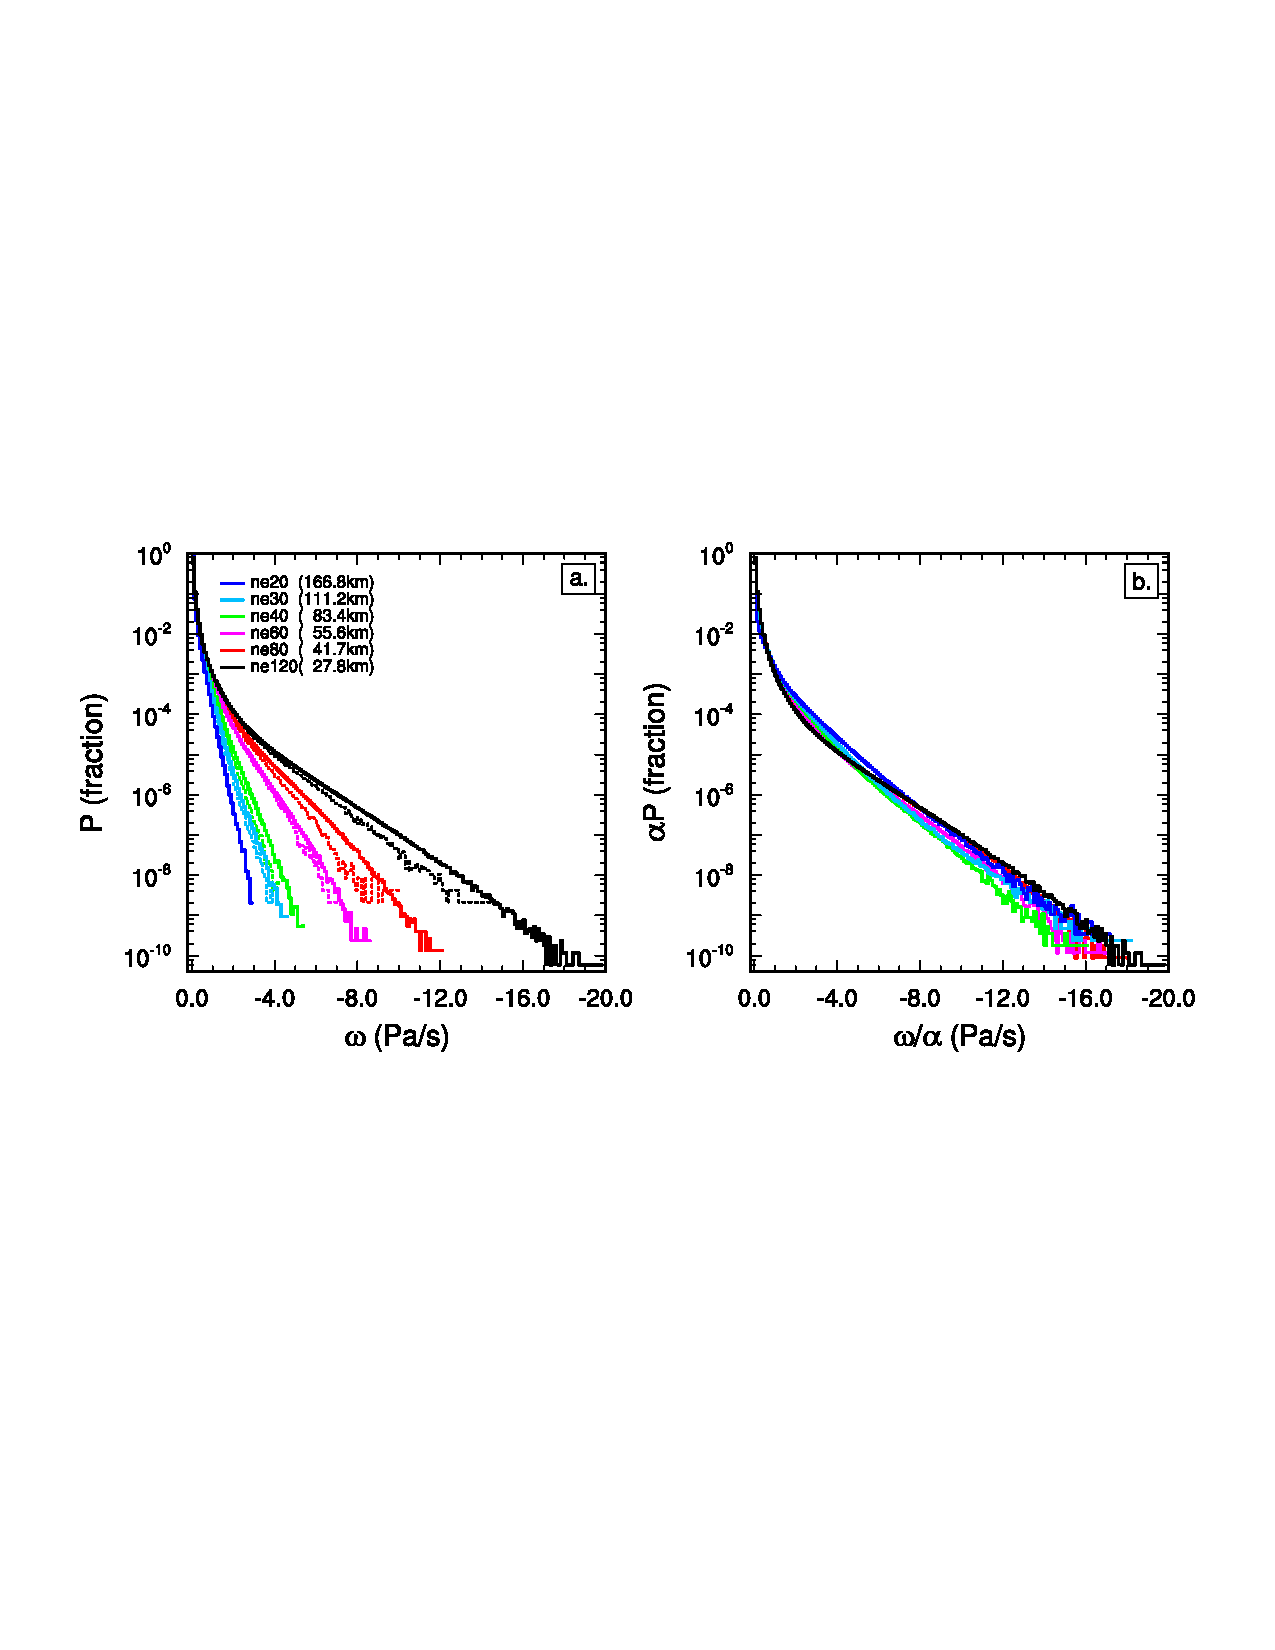
\includegraphics[width=20pc,angle=0]{figs/temp_2pdf.pdf}\\
\end{center}
\caption{Probability density distribution of the upward vertical pressure velocities $\omega$ computed everywhere in the model from six-hourly output over the entirety of the year-long simulations. (a) Values on their native grid (solid) and values bilinearly remapped to the $ne20$ grid (dotted), (b) values on their native grid, scaled to the $ne120$ resolution using a power law exponent $n=-1$ in equation~\ref{eq:alpha}.}
\label{fig:2pdf}
\end{figure}

The probability density function (PDF) of negative, or upward vertical pressure velocities $\omega$ in the aqua-planets is provided in Figure~\ref{fig:2pdf}a. The magnitude of upward $\omega$ increases monotonically with resolution, with positive, or downward $\omega$ behaving similarly (not shown). This monotonic increase in the magnitude of $\omega$ is evident even after remapping all model output to a common grid ($ne20$; dotted curves in Figure~\ref{fig:2pdf}a).

The PDF's may be scaled to the highest-resolution resolution grid through $ \alpha P (\omega / \alpha)$, where $P(x)$ is the PDF, and $\alpha$ the scale factor from equation~\ref{eq:alpha} with $\Delta x_0$ set to the $ne120$ grid-spacing. Figure~\ref{fig:2pdf}b shows the scaled PDF's for a power law exponent $n=-1$ in $\Delta x$. The scaled PDF's all collapse onto the high-resolution reference, indicating that the power-law exponent $n=-1$ explains to first-order the variation in vertical velocity with resolution as shown by the aqua-planet simulations. 

Changes to the vertical velocity field can be further understood through decomposing the mass weighted vertical mean $ \langle \omega \rangle$ into upward and downward components,
\begin{equation}
\langle \omega \rangle =\langle f_{u} \rangle \, \langle \omega_{u} \rangle + \langle f_{d} \rangle \, \langle \omega_{d} \rangle, \label{eq:omega}
\end{equation}
where $\langle f_x \rangle$ and $\langle \omega_x \rangle$ refers to the vertical mass fraction $ \left( \frac{\int dp_x}{\int dp} \right)$ and the $x$ component of the mass weighted vertical mean of $\omega$ $ \left( \frac{\int \omega_x dp_x}{\int dp_x} \right)$, respectively, subscript $u$ refers to upward motion and $d$, downward motion.

The global mean, climatological components $\langle f_{u} \rangle \, \langle \omega_{u} \rangle$ and $\langle f_{d} \rangle \, \langle \omega_{d} \rangle$ are provided in Figure~\ref{fig:2panel}a,b for the aqua-planet simulations. The magnitude of both $\langle f_{u} \rangle \, \langle \omega_{u} \rangle$ and $\langle f_{d} \rangle \, \langle \omega_{d} \rangle$ increase monotonically with resolution, and are equal and opposite, which is a requirement of mass conservation in the model and a convenient check of the calculation. While $\langle f_{d} \rangle$ is about 25\% larger than $\langle f_{u} \rangle$ in all simulations, the vertical mass fractions vary by only few percent with resolution, and so the monotonic behavior of $\langle f_{x} \rangle \, \langle \omega_{x} \rangle$ with resolution is primarily from variations in $ \langle \omega_{x} \rangle$ (not shown).

\begin{figure}
\begin{center}
\noindent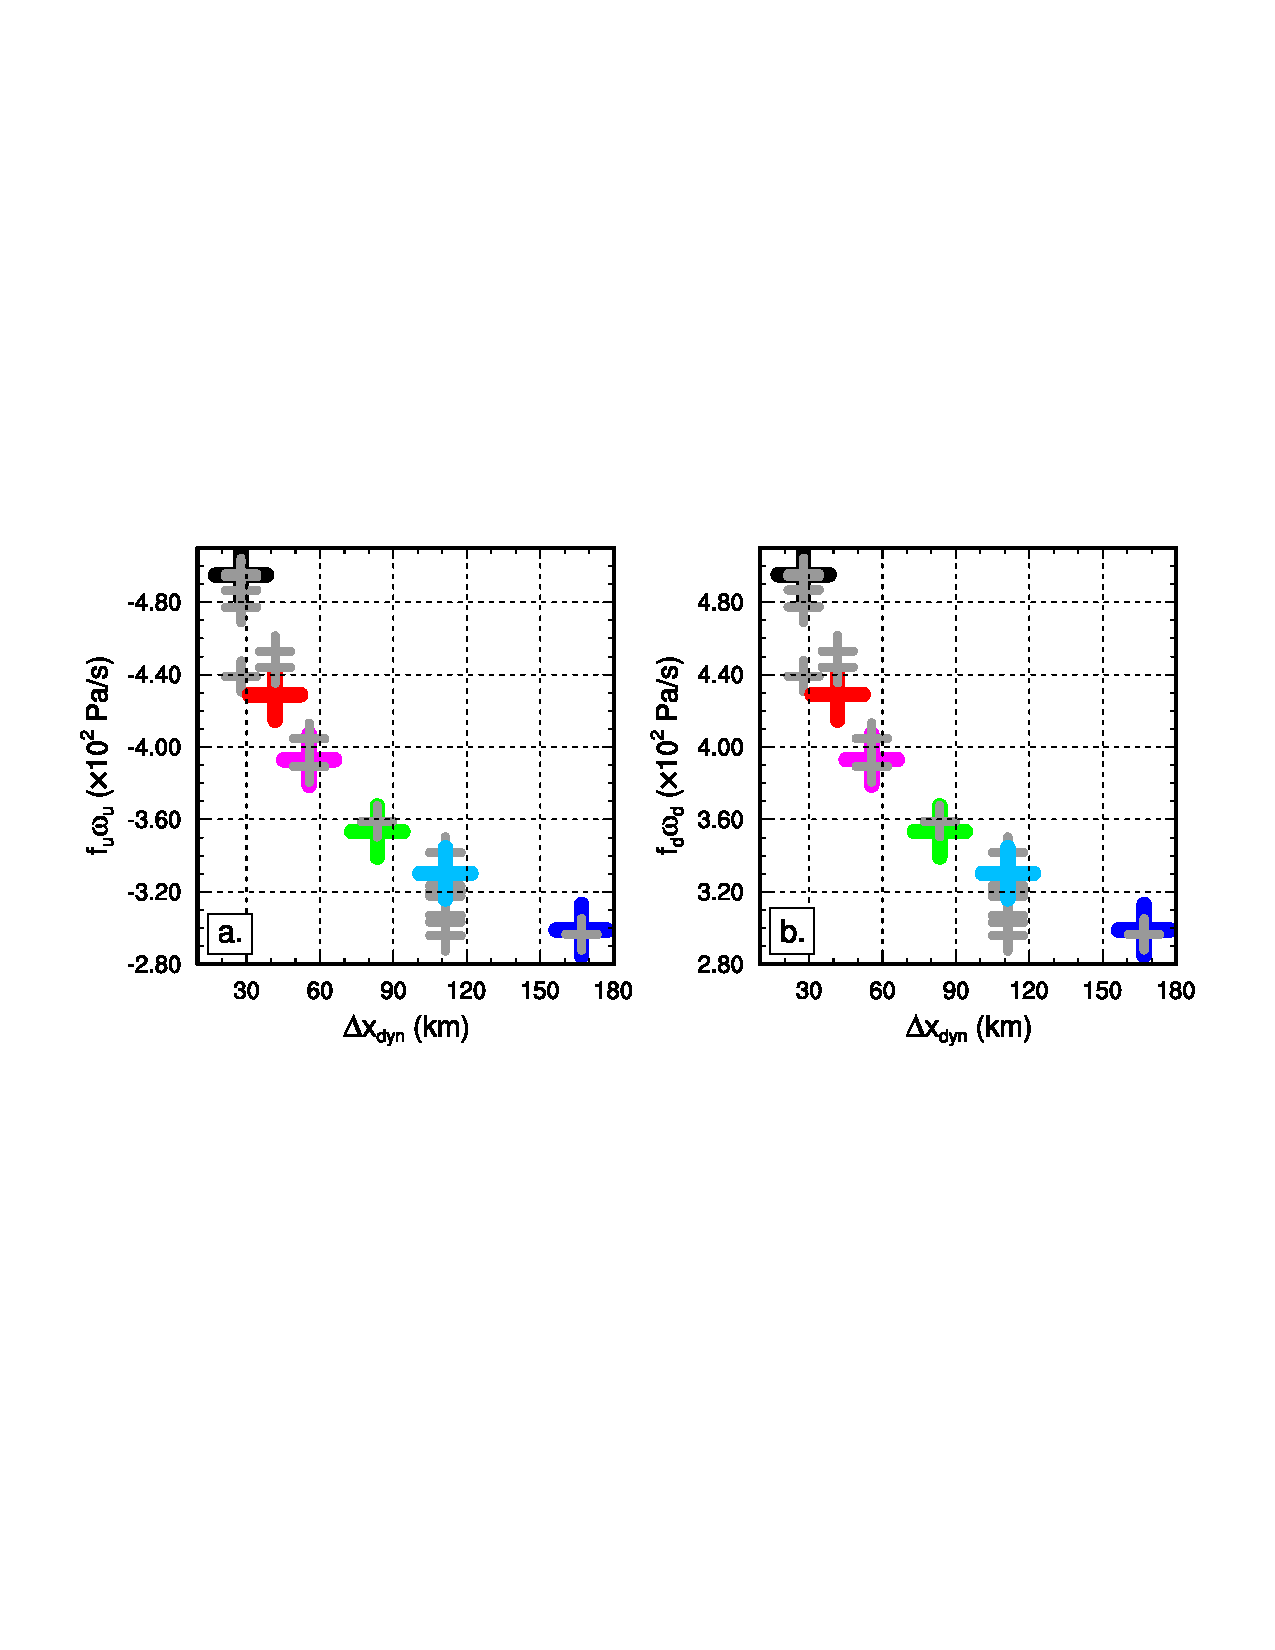
\includegraphics[width=20pc,angle=0]{figs/temp_diags_2panel.pdf}\\
\end{center}
\caption{Components of the climatological, global mean vertical pressure velocity, (a) $\langle f_{u} \rangle \langle \omega_{u} \rangle$ and (b) $\langle f_{d} \rangle \langle \omega_{d} \rangle$. Grey crosses are for the 24 member perturbed parameter ensemble.}
\label{fig:2panel}
\end{figure}

\subsection{Vertical Velocities and Deep Convective Precipitation}

The large increase in magnitude of the upward and downward vertical velocities with resolution may be expected to impact the behavior of other model components. Curiously, there is an excellent negative correlation (Pearson's R-value = 0.99, N = 27) between the global mean, climatological $\langle f_{d} \rangle \, \langle \omega_{d} \rangle$ and a measure of the activity of the \cite{ZM1995AO} deep convection scheme (referred to as the {\em{ZM scheme}} hereafter), global mean, climatological $FREQZM$ (Figure~\ref{fig:corr}). At any grid-point and time-step, $FREQZM$ is a binary variable: 1 if the ZM scheme is active, 0 if it is not. Time mean $FREQZM$ is therefore the fraction of the model time that the ZM scheme is triggered, i.e., dilute CAPE exceeds $\geq 70$ J/kg. The regression indicates that model simulations with greater subsidence also have less convective activity.

\begin{figure}
\begin{center}
\noindent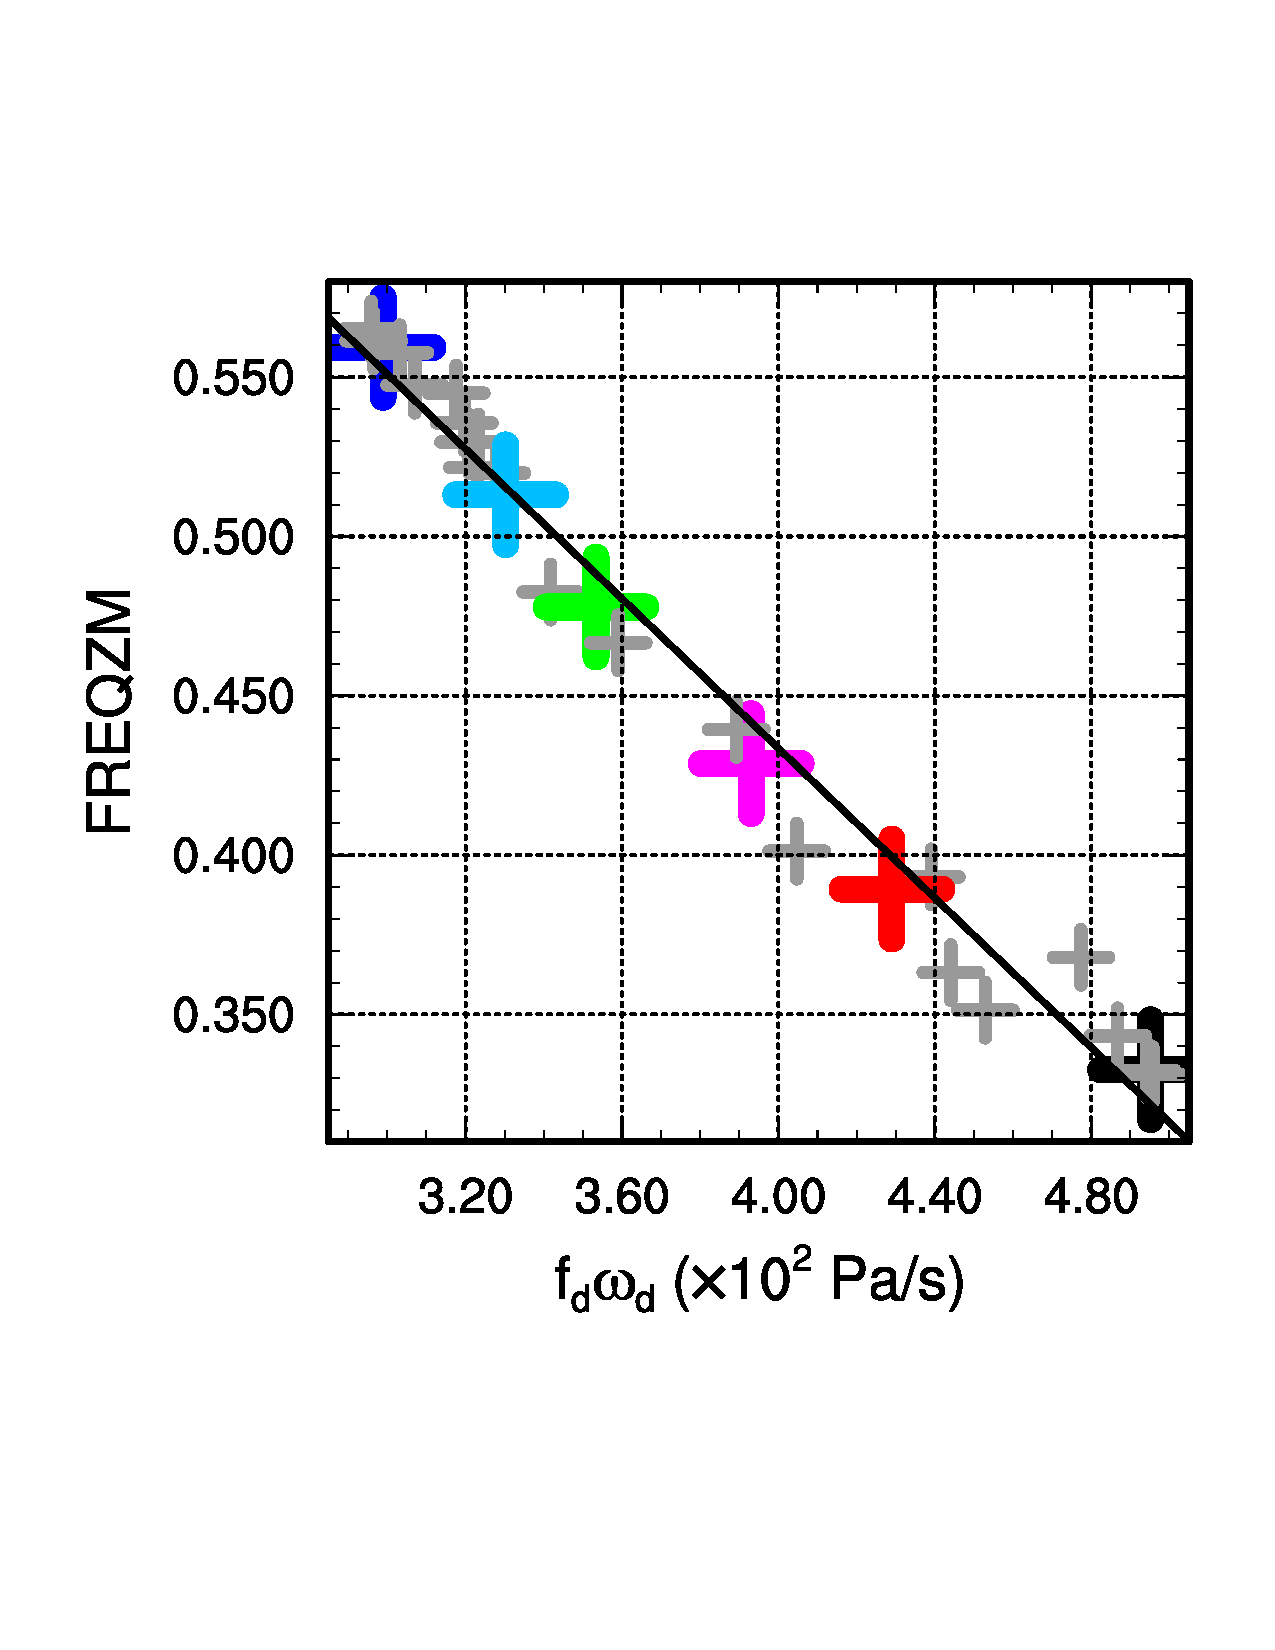
\includegraphics[width=20pc,angle=0]{figs/temp_diags_corr.pdf}\\
\end{center}
\caption{Scatter plot of global mean, climatological $\langle f_{d} \rangle \langle \omega_{d} \rangle$ and FREQZM, and the fitted linear regression which has a Pearson's R-value = 0.99, using all 27 simulations. Grey crosses are for the 24 member perturbed parameter ensemble runs.}
\label{fig:corr}
\end{figure}

Figure~\ref{fig:4zonal}a,b, shows the zonal mean variations in $\langle f_{d} \rangle \, \langle \omega_{d} \rangle$ and $FREQZM$ in the convergence experiment. $FREQZM$ is largest in the $\pm 10^{\circ}$ latitude region, within the Intertropical Convergence Zone (ITCZ), and rapidly decreasing polewards into the subtropics. $\langle f_{d} \rangle \, \langle \omega_{d} \rangle$ increases away from the ITCZ region and reaches a maximum at the poleward limit of the Hadley Cell. The increase (decrease) in $\langle f_{d} \rangle \, \langle \omega_{d} \rangle$ ($FREQZM$) with resolution is to first-order, independent of latitude.

\begin{figure}
\begin{center}
\noindent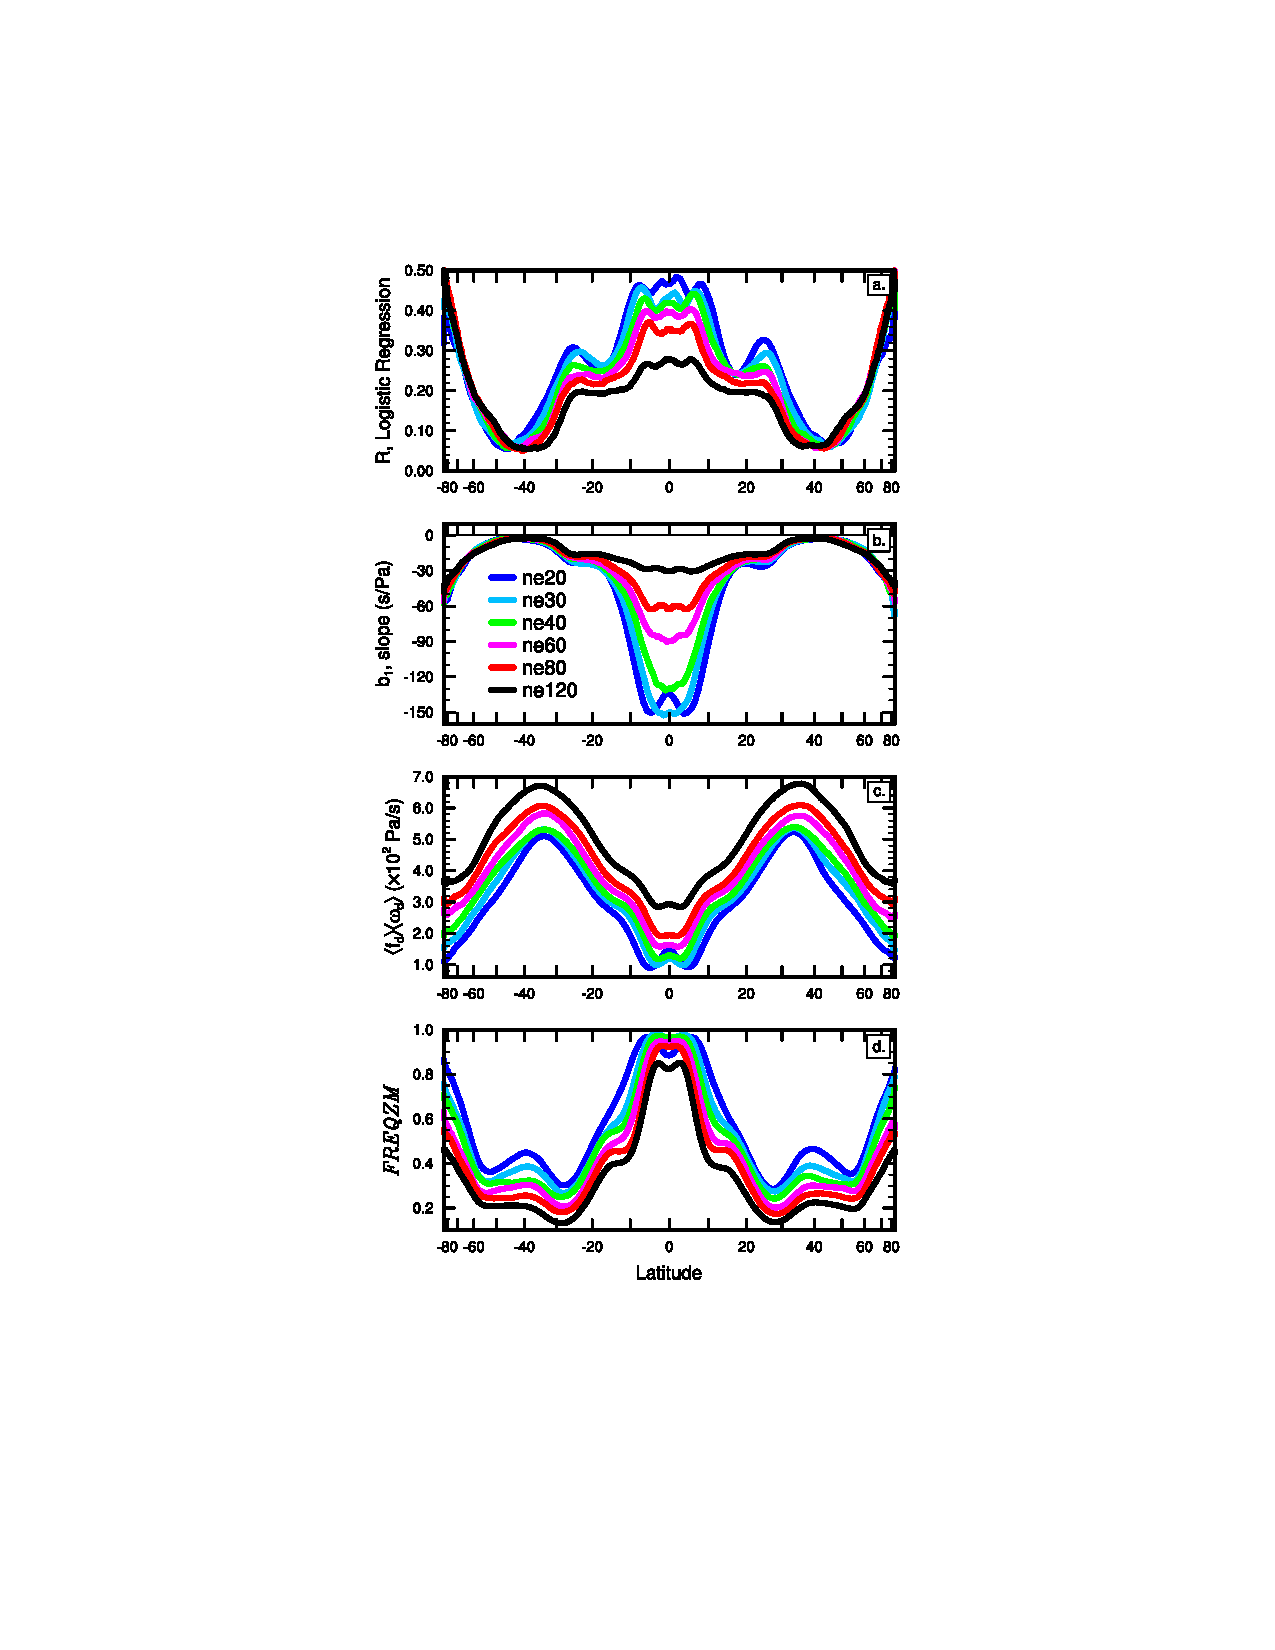
\includegraphics[width=14pc,angle=0]{figs/temp_4zonal.pdf}\\
\end{center}
\caption{Zonal mean (a) climatological $\langle f_{d} \rangle \langle \omega_{d} \rangle$ and (b) climatological $FREQZM$. Zonal mean (c) R-values and (d) the shape parameter $b_1$ in the logistic regression.}
\label{fig:4zonal}
\end{figure}

To further understand the relationship between subsidence and activity of the ZM scheme, a logistic regression between $\langle f_{d} \rangle \langle \omega_{d} \rangle$ and $FREQZM$ is performed for each grid column within each of the simulations. Logistic regression uses an iterative method to fit a continuous variable predictor, $x$ to a binary predictand $p$ using the exponential \citep{WILKSBOOK},
\begin{equation}
p = \frac{exp{[b_0 + b_1 x]}}{1 + exp{[b_0 + b_1 x]}}, \label{eq:logreg}
\end{equation}
where $b_0$ and $b_1$ are the shape parameters of the exponential. The predictor is the instantaneous $\langle f_{d} \rangle \langle \omega_{d} \rangle$ of a grid column, and the predictand the binary $FREQZM$. The assumption is then that subsidence is the independent variable, which is reasonable considering the environment of subsiding regions is generally more stable than its surroundings, and the ZM scheme is modulated by the dilute CAPE stability calculation. Grid column regressions that are statistically significant at the $95\%$ level using a log-likelihood test \citep{WILKSBOOK} are retained for analysis. Since the aqua-planets have zonally symmetric boundary conditions, there is a zonally varying structure in the goodness of fit (R-value) and shape parameter $b_1$ (Figure~\ref{fig:4zonal}c,d).

The zonal mean R-values indicate the greatest goodness of fit in the $\pm 10^{\circ}$ latitude band, hereafter referred to as the deep tropics. In this region, the shape parameter $b_1$ is large and negative (Figure~\ref{fig:4zonal}d), consistent with the idea that subsiding motion stabilizes the environment and actively depresses dilute CAPE and the activity of the ZM scheme in the simulations. The shape parameter becomes less negative in the deep tropics with resolution, likely due to the greater magnitude $\langle f_{d} \rangle \langle \omega_{d} \rangle$ with resolution, which requires a lower $b_1$ to predict the binary $FREQZM$. The R-values generally decrease with resolution indicating that there is degradation in the relationship with resolution.

\subsubsection{Deep Tropics}

Table~\ref{tbl:table2} shows the fractional contribution of the deep tropics to the climatological, global mean change in convective precipitation with resolution. The table indicates that a majority ($60-70 \%$) of the reduction in convective precipitation with resolution is from changes within the deep tropics (except in going from $ne20$ to $ne30$, where convective precipitation rates increase, in part due to a wide double-ITCZ in the $ne20$ run that spans outside of $\pm 10^{\circ}$ latitude, but which is contained within $\pm 10^{\circ}$ latitude in the $ne30$ run). Expanding the latitude boundaries marginally to $\pm 15^{\circ}$, roughly $75\%$ of the changes in convective precipitation with resolution occurs in this region (again, ignoring $ne30-ne20$; Table~\ref{tbl:table2}). This trend reflects changes in the partitioning of the ITCZ from convective to stratiform precipitation with resolution. 

The large reduction in convective precipitation with resolution in the deep tropics also happens to be the region where the logistic regression indicates that subsiding motion is most skillful at depressing the activity of the convection scheme. But the change in $FREQZM$ in the deep tropics with resolution is not substantially different from any other region (Figure~\ref{fig:4zonal}b), such as the midlatitudes where the logistic regression indicates a poor relationship between subsidence and $FREQZM$ (Figure~\ref{fig:4zonal}c). The deep tropics is then only unique for its substantially larger change in ZM precipitation per change in $FREQZM$ with resolution.

 \begin{table}
 \caption{Fractional contribution of latitude bands $\pm 10^{\circ}$ and $\pm 15^{\circ}$ to changes in global mean precipitation with resolution. The grid headers refer to differences with respect to the next lowest grid resolution, e.g., $ne30 = ne30-ne20$, $ne40=ne40-ne30$, etc... All differences are computed after conservative remapping to a common $ne20$ grid.}
 \centering
 \scriptsize
 \begin{tabular}{lcccccc}
   \hline
   Variable & $ne30$ & $ne40$ & $ne60$ & $ne80$ & $ne120$ \\ 
   \hline
   $\pm 10^{\circ}$ ($17.6\%$ of global area) \\
   Convective Precipitation & -0.58 & 0.62 & 0.66 & 0.72 & 0.70 \\
   Stratiform Precipitation & 0.55 & 0.63 & 0.69 & 0.67 & 0.41 \\ 
   \hline
   $\pm 15^{\circ}$ ($25.8\%$ of global area) \\
   Convective Precipitation & 0.22 & 0.75 & 0.73 & 0.79 & 0.72 \\
   Stratiform Precipitation & 0.46 & 0.64 & 0.71 & 0.70 & 0.49 \\      
 \hline
 \end{tabular}
 \label{tbl:table2}
 \end{table}

To characterize the changes to dilute CAPE of subsiding regions in the deep tropics with resolution, temperature and moisture profiles are conditionally sampled depending on whether $\langle \omega \rangle$ is positive or negative, indicating predominantly subsiding or ascending grid columns. The time mean temperature and moisture profiles of subsiding and ascending regions are then used to compute the dilute CAPE used in the ZM scheme, offline. Figure~\ref{fig:cape}a shows the dilute CAPE values associated with mean conditions for ascending, descending and all grid columns in the deep tropics, with resolution. Ascending regions are associated with larger values of dilute CAPE ($>180$ J/kg) relative to subsiding regions ($<110$ J/kg), and the dilute CAPE in both regimes decreases monotonically with resolution. 

\begin{figure}
\begin{center}
\noindent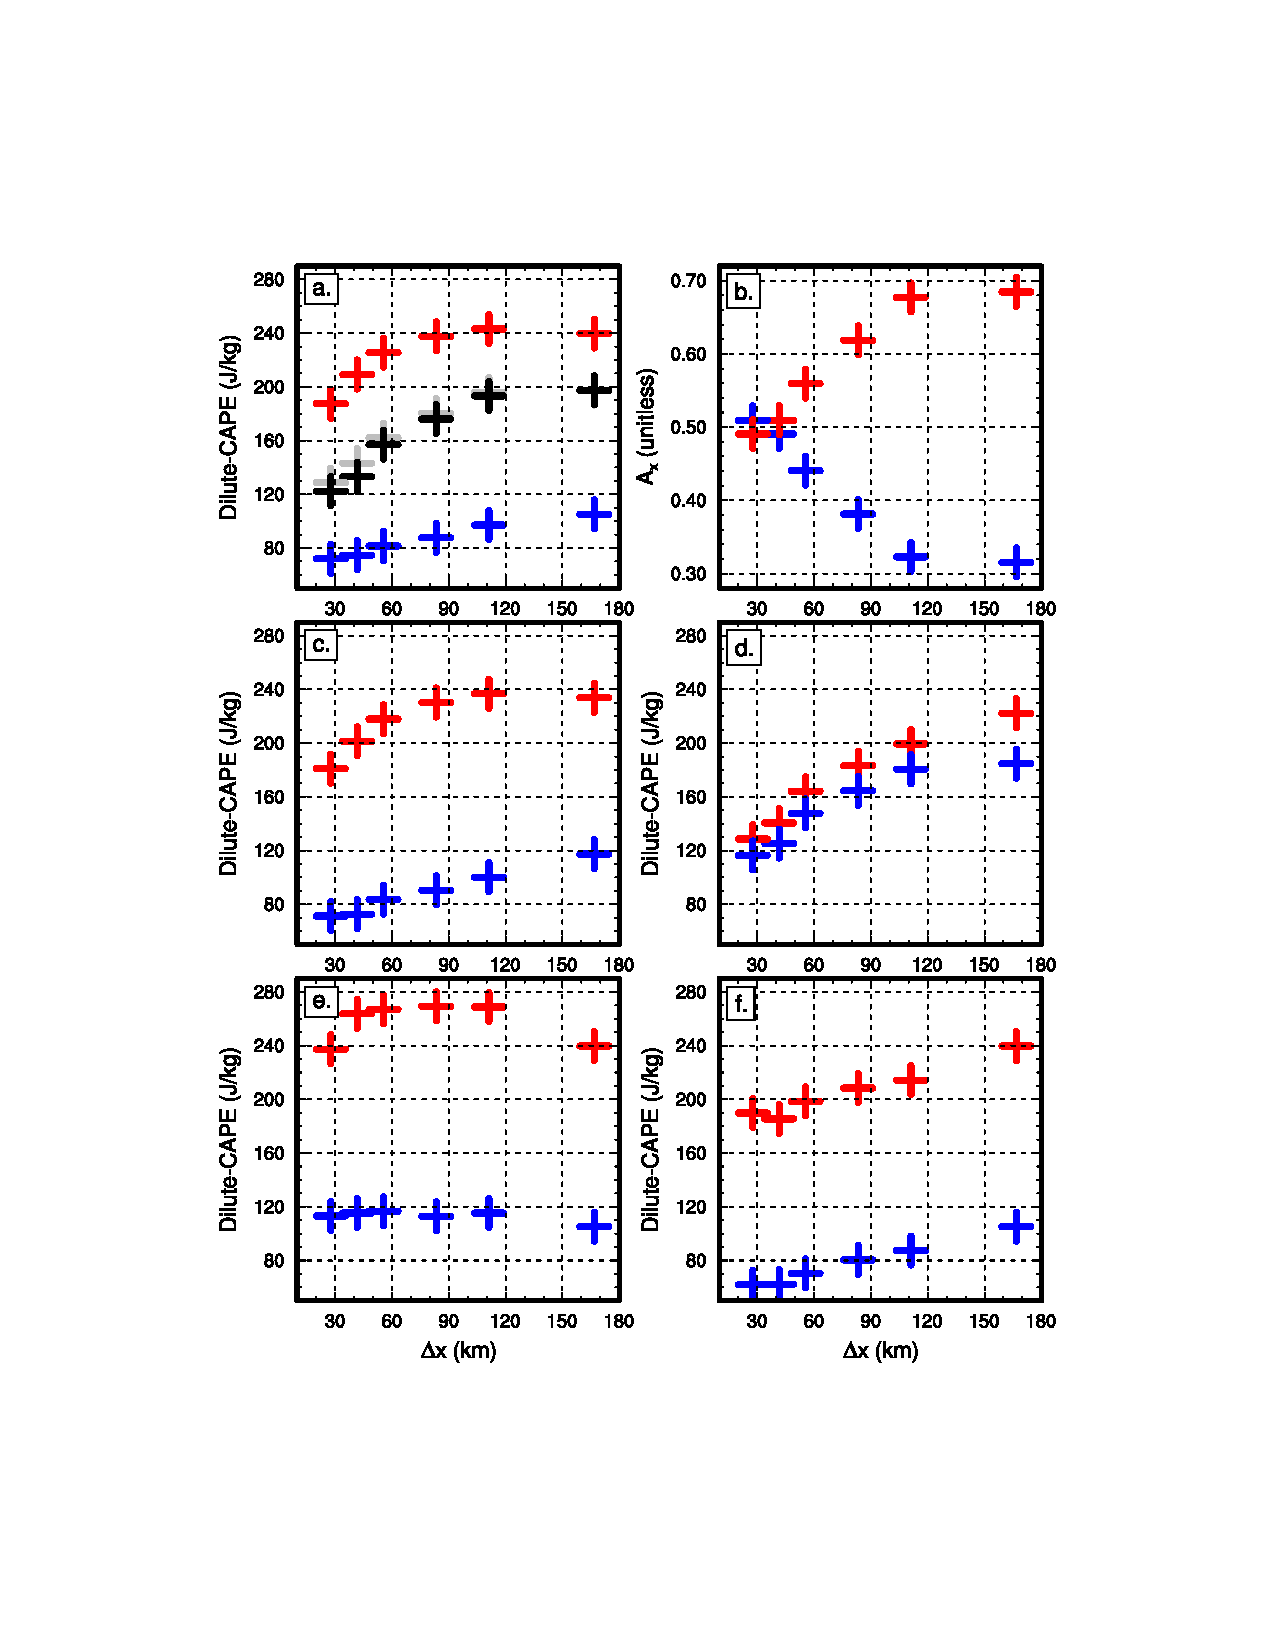
\includegraphics[width=20pc,angle=0]{figs/temp_cape.pdf}\\
\end{center}
\caption{(a) Dilute CAPE computed from time mean temperature and moisture profiles of ascending (red), subsiding (blue) and all grid columns (black) in the deep tropics ($\pm 10^{\circ}$ latitude), and (b) space-time weights of ascending (red) and descending (blue) grid columns in the deep tropics. (c) Dilute CAPE computed for ascending/descending grid columns, but using the mean temperature profile for the entire deep tropics, and (d) Dilute CAPE for ascending/descending regions but fixing moisture to the $ne20$ profile. Grey crosses in (a) are dilute CAPE derived from the sum of the products of space-time weights with the dilute CAPE values of ascending/descending grid columns.}
\label{fig:cape}
\end{figure}

Figure~\ref{fig:profiles} shows the time mean temperature and specific humidity profiles of subsiding grid cells in the deep tropics, expressed as anomalies from the mean temperature and specific humidity of the entire deep tropics. The mean profiles of subsiding regions have an anomalous warming layer in the $600-800$ hPa layer and an anomalous moisture deficit throughout the entire column. This warming and drying pattern is consistent with the effects of subsidence, whose motion adiabatically warms the environment while simultaneously advecting drier conditions aloft, downward. Both warming and drying the environment oppose the growth of dilute CAPE through reducing parcel buoyancy; warming the environment relative to the temperature of rising air parcels reduces parcel buoyancy \citep{Z2002JGR}, and mixing drier environmental air into rising air parcels reduces the moisture available to warm parcels through latent heating \citep{RB1992JAS}.

\begin{figure}
\begin{center}
\noindent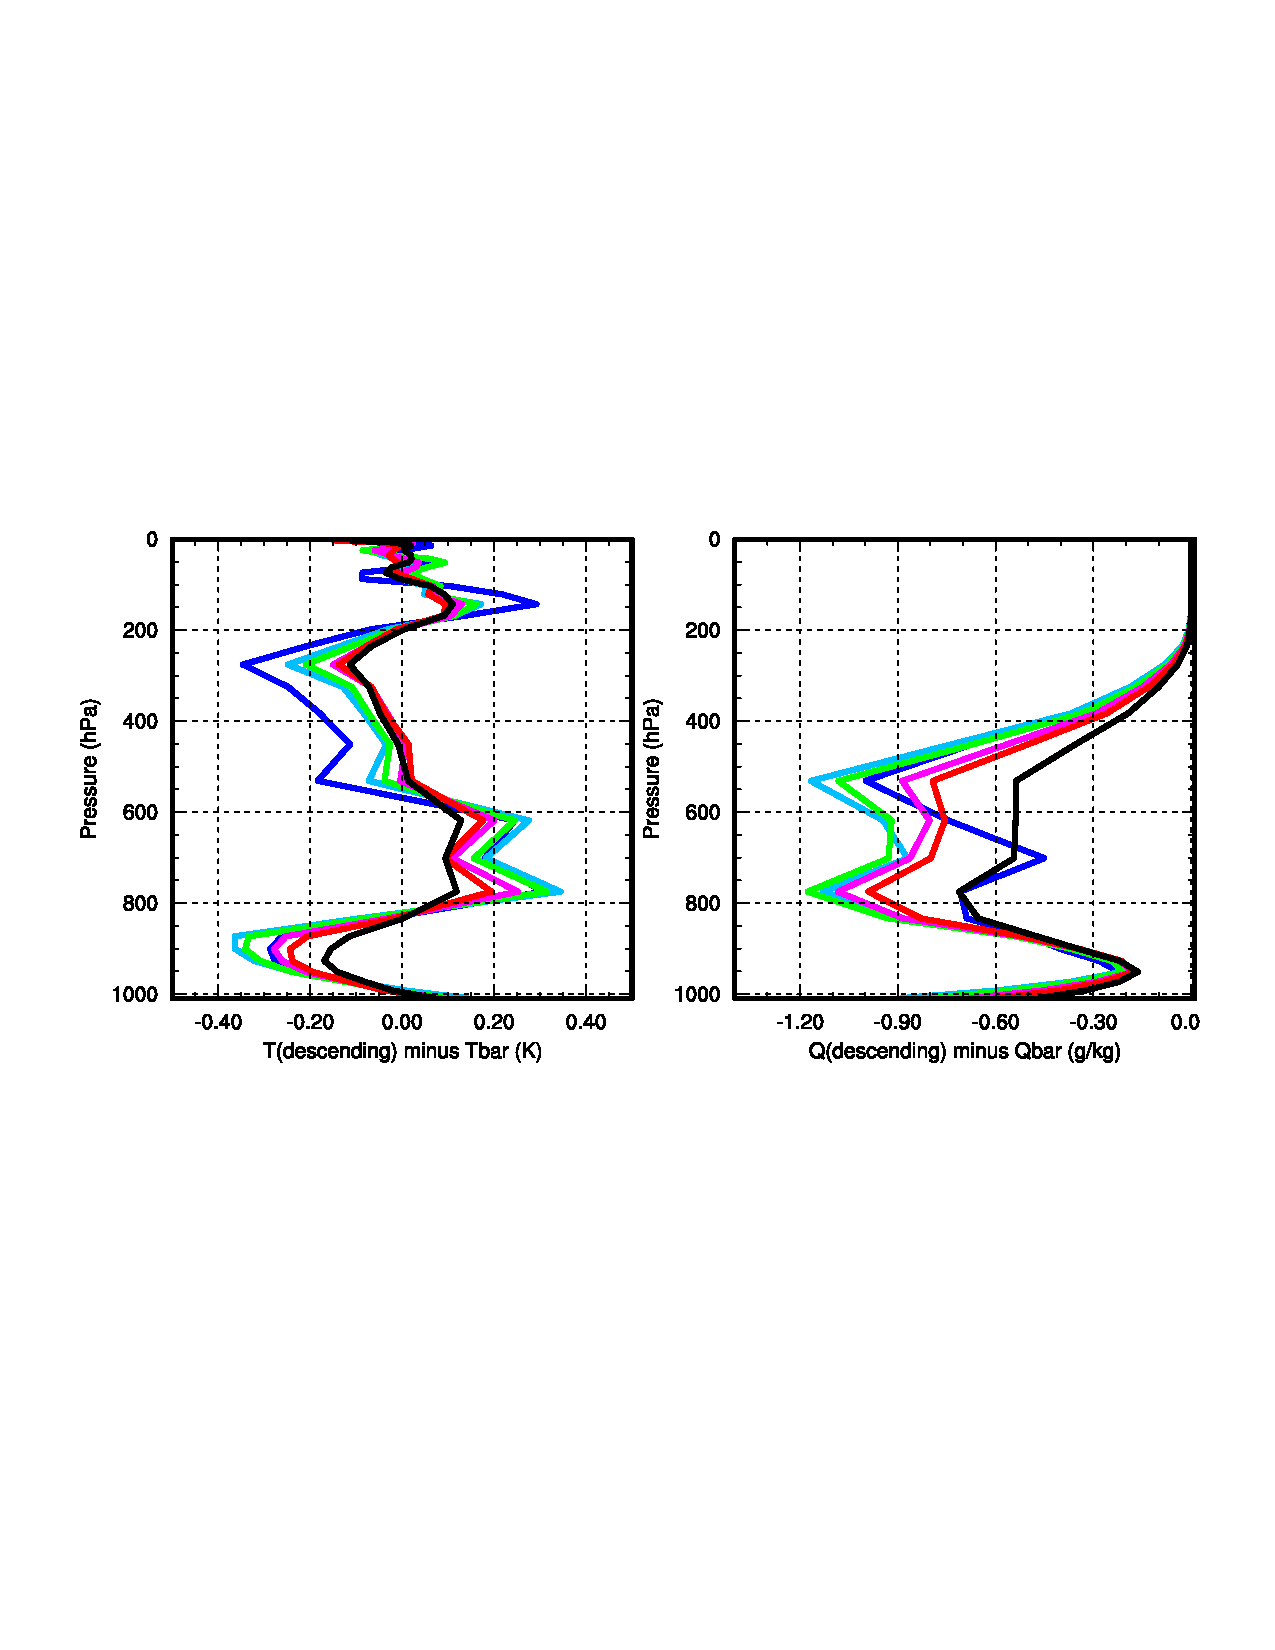
\includegraphics[width=20pc,angle=0]{figs/temp_profiles.pdf}\\
\end{center}
\caption{Time mean (a) temperature and (b) specific humidity profiles of subsiding grid cells in the deep tropics ($\pm 10^{\circ}$ latitude) in the convergence experiment, presented as anomalies from the mean temperature and specific humidity of the entire deep tropics in each simulation.}
\label{fig:profiles}
\end{figure}

The large spread in dilute CAPE between ascending/descending regions is crucial for maintaining the relationship shown by the logistic regression, since the much smaller values of dilute CAPE of subsiding grid columns is required to depress dilute CAPE below the threshold for convection. To unravel the contributions of warming and drying shown in Figure~\ref{fig:profiles} to the large spread in dilute CAPE between the two regimes, dilute CAPE is recomputed using the mean specific humidity of ascending/descending regions in the deep tropics, but setting the temperature profile to the mean profile for the entire deep tropics. Figure~\ref{fig:cape}c shows this influence of changing moisture on dilute CAPE, which to first order, explains the large spread in dilute CAPE between the ascending/descending regions in the deep tropics. Temperature differences between ascending/descending regimes has a smaller, second order influence on the spread in dilute CAPE (not shown).

The space-time weights associated with ascending and descending grid columns in the deep tropics vary drastically with resolution (Figure~\ref{fig:cape}b). The subsiding (ascending) space-time weights change from $0.32$ ($0.68$) in the $ne20$ run, monotonically increasing (decreasing) with resolution to $0.51$ ($0.49$) in the $ne120$ run. This increasing occurrence of stable, subsiding grid columns accounts for about half of the changes in dilute CAPE in the deep tropics with resolution, the other half being due to the systematic reduction in dilute CAPE for both ascending and descending regions (Figure~\ref{fig:cape}a). This is verified through comparing the weighted sum of the ascending/descending dilute CAPE values with the dilute CAPE for the entire deep tropics (compare black and grey crosses in Figure~\ref{fig:cape}a). 

To isolate the relative importance of temperature or moisture on the systematic reduction in dilute CAPE with resolution for both ascending/descending regimes, dilute CAPE is recomputed for all resolutions, but through fixing the moisture profiles to the lowest resolution $ne20$ profile, and then through only fixing only the temperature to the $ne20$ profile. Figure~\ref{fig:cape}d shows the influence of changing temperature profile with resolution on dilute CAPE of ascending/descending grid columns, and illustrates that the systematic reduction in dilute CAPE with resolution in both regimes is primarily from changes to the temperature field. Moisture changes with resolution has a smaller influence, only appreciably impacting the dilute CAPE of ascending regions at higher resolutions (not shown).

\subsubsection{Subtropics}

Figure~\ref{fig:cape-subt}a shows the dilute CAPE values computed from mean temperature and moisture of subsiding and ascending regions in the $\pm \left( 10^{\circ}-30^{\circ} \right) $ latitude bands, hereafter referred to as the subtropics. The spread in dilute CAPE between ascending and descending grid columns is much smaller than for the deep tropics (Figure~\ref{fig:cape}a), and their dilute CAPE  values vary much less with resolution ($\sim 20$ J/kg, compared with $\sim 80$ J/kg across all resolutions in the deep tropics). Through recomputing dilute CAPE and fixing the temperature or moisture profiles to $ne20$ values, the reduction in dilute CAPE with resolution is attributed to both temperature and moisture, but with temperature changes playing a larger role (not shown). This analysis suggests that Increasing subsidence with resolution increases the stability of the mean state, since both ascending/descending regimes become more stable with resolution, and reducing climatological $FREQZM$ despite the poor relationship between instantaneous subsidence and $FREQZM$ in the subtropics, as shown by the logistic regression (Figure~\ref{fig:4zonal}c).

\begin{figure}
\begin{center}
\noindent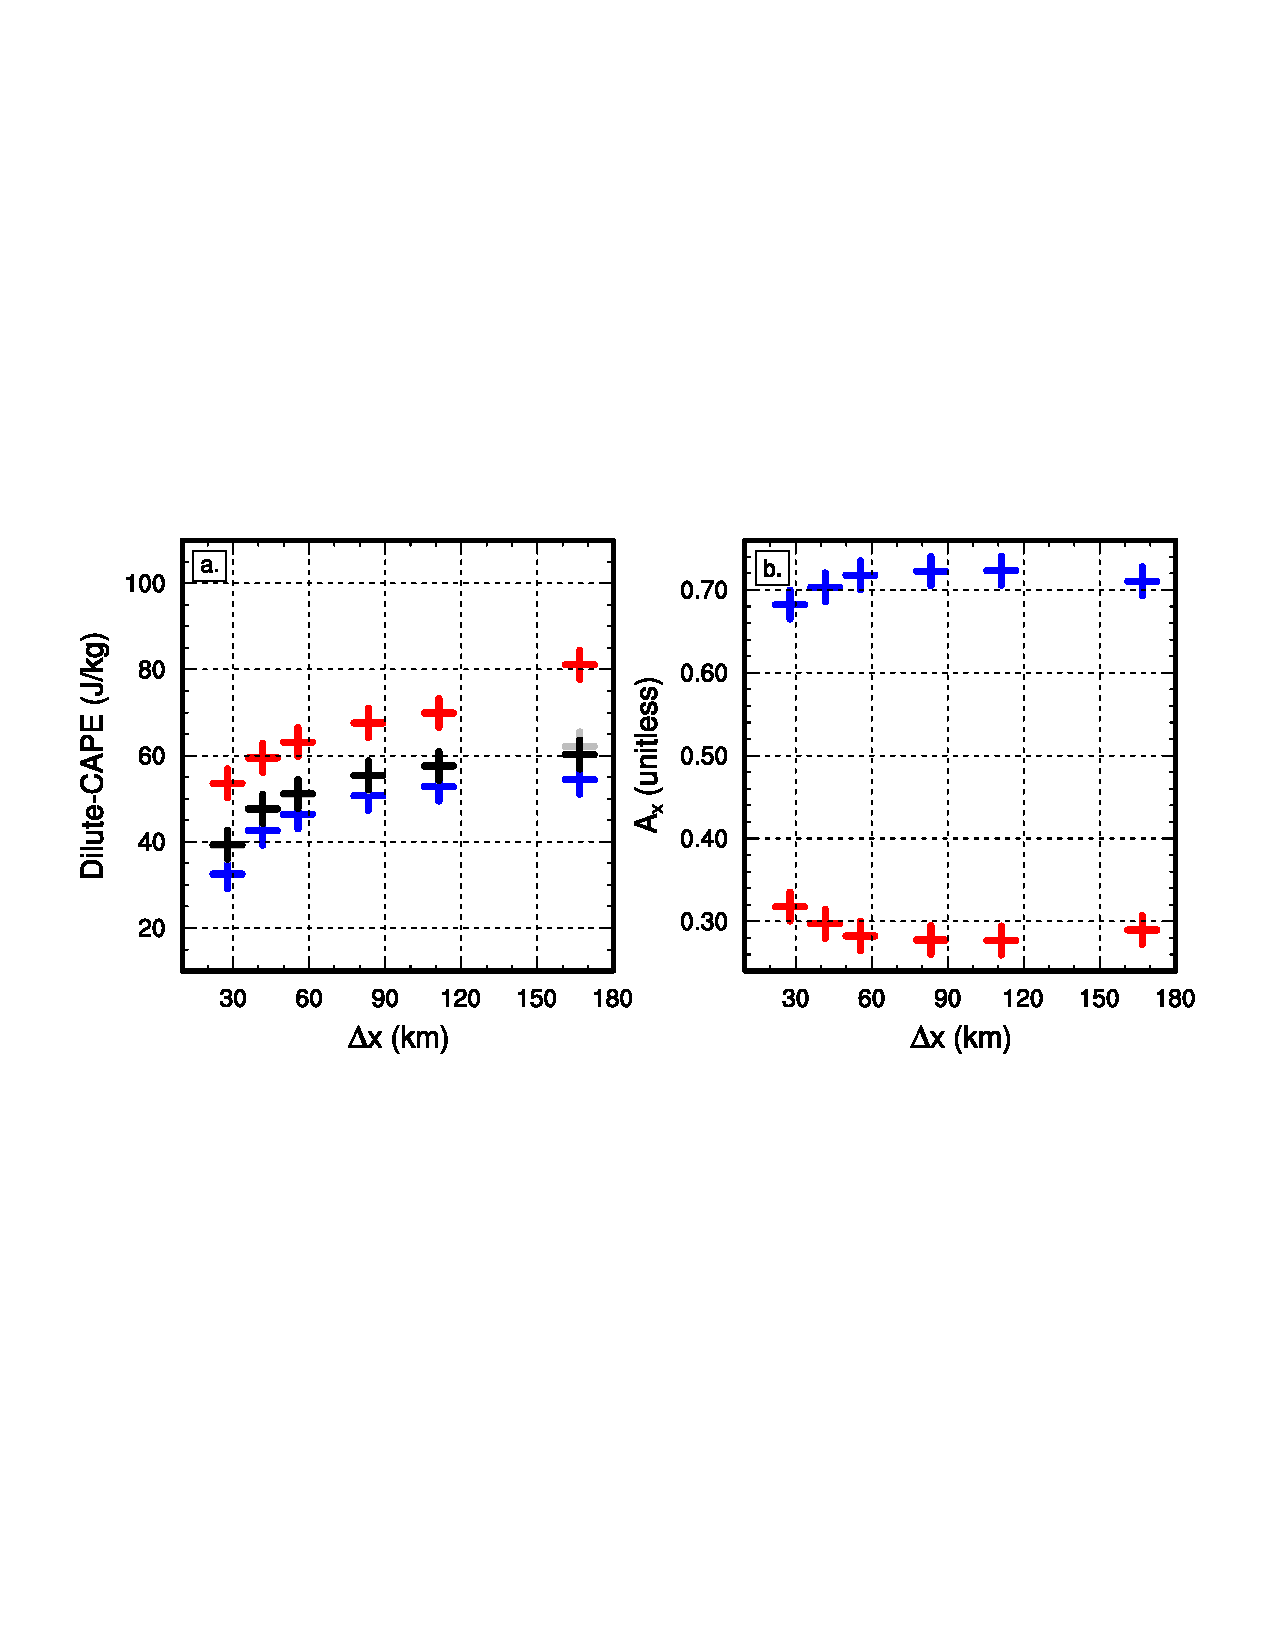
\includegraphics[width=20pc,angle=0]{figs/temp_cape-subtropics.pdf}\\
\end{center}
\caption{(a) Dilute CAPE computed from time mean temperature and moisture profiles of ascending (red), subsiding (blue) and all grid columns (black) in the subtropics ($\pm \left(10^{\circ}-30^{\circ} \right)$ latitude bands), and (b) space-time weights of ascending (red) and descending (blue) grid columns in the subtropics. Grey crosses in (a) are dilute CAPE derived from the sum of the products of space-time weights with the dilute CAPE values of ascending/descending grid columns.}
\label{fig:cape-subt}
\end{figure}

It is the lack of spread in dilute CAPE between ascending/descending regions that explains the declining skill in the logistic regression in the subtropics (Figure~\ref{fig:4zonal}c). Without a strong dependence of dilute CAPE on ascending/descending regimes, subsidence is not a very skillful predictor of depressing dilute CAPE below the threshold for convection. In contrast to the deep tropics, there is also no significant changes to the occurrence of subsiding grid columns with resolution; space-time weights of ascending/descending motion are more-or-less invariant with resolution (Figure~\ref{fig:cape-subt}b).

\begin{figure}
\begin{center}
\noindent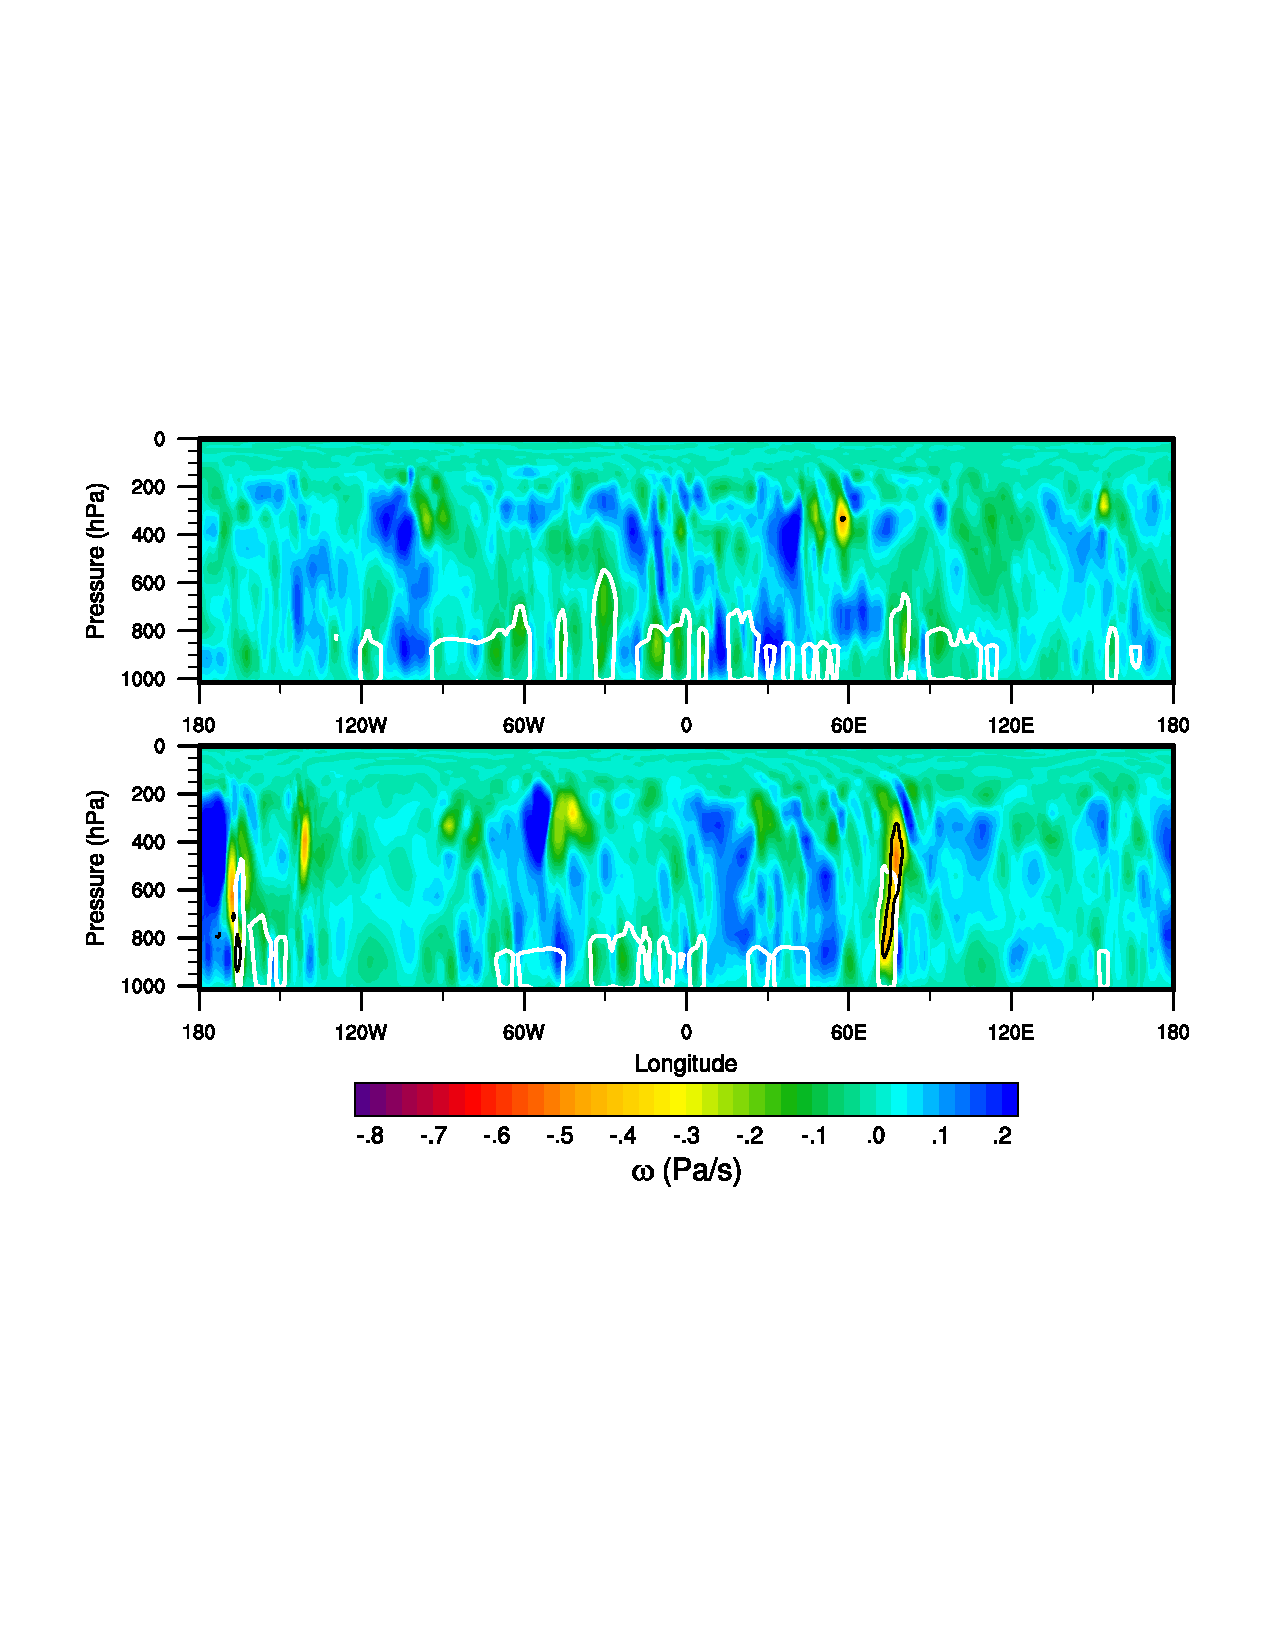
\includegraphics[width=20pc,angle=0]{figs/temp_trans.pdf}\\
\end{center}
\caption{(a,b) Two snapshots of $\omega$ for a longitude-pressure transect at $\sim 18^{\circ}$ latitude in the $ne30$ simulation, overlain by the $0.0075$ kg/m$^2$/s contour of the ZM mass flux (white) delineating the region where the ZM scheme is active, and the 15 K/day contour of the total physics tendencies (black), indicating stratiform cloud formation.}
\label{fig:transect}
\end{figure}

To understand why dilute CAPE is less sensitive to subsidence in the subtropics, Figure~\ref{fig:transect} shows two snapshots of $\omega$ in the longitude-pressure plane at  $\sim 18^{\circ}$ latitude in the $ne30$ simulations, overlain by an isoline delineating where the ZM mass fluxes are quite active. The ZM mass fluxes typically only extend up to about the 800 hPa level in this region, which often occurs with appreciable subsiding motion aloft. Though properly a deep convection scheme, the ZM scheme is acting as a shallow convection scheme in this region. This shallow convection regime tends to produce light rain, or drizzle, which is a common bias in AGCMs \citep{D2006JCLIM}. Figure~\ref{fig:2zonal}a shows the fraction of ZM precipitation $\leq 5$ mm/day in the simulations, which stubbornly persists at $\sim$ 70\% in the $\pm \left(10^{\circ}-20^{\circ} \right)$ latitude bands, irrespective of resolution.

\begin{figure}
\begin{center}
\noindent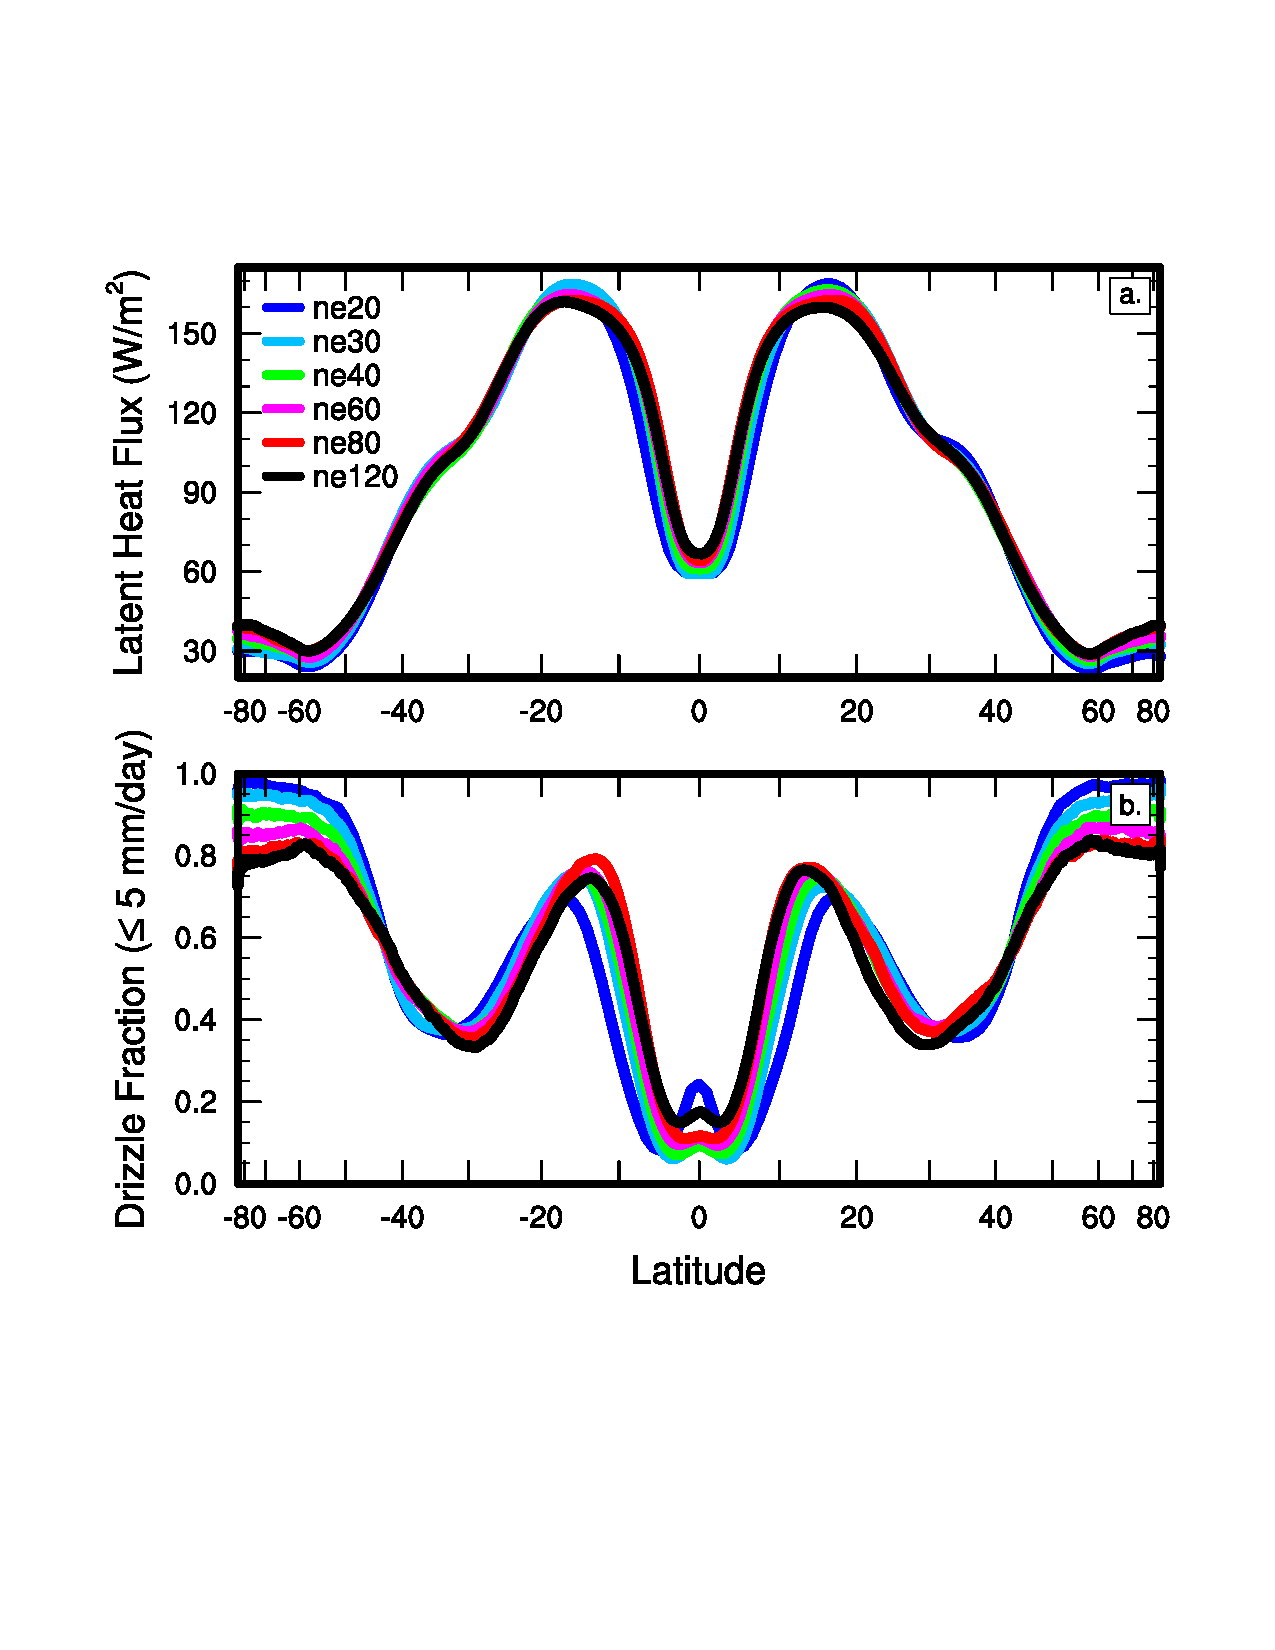
\includegraphics[width=14pc,angle=0]{figs/temp_2zonal.pdf}\\
\end{center}
\caption{Climatological zonal mean (a) drizzle fraction and (b) surface latent heat fluxes in the convergence experiment. Drizzle fraction is defined as sum  convective precipitation rates $\leq 5$ mm/day divided by the sum of all convective precipitation rates, computed from 6-hourly instantaneous fields over the duration of the simulation.}
\label{fig:2zonal}
\end{figure}

In the $\pm \left(10^{\circ}-20^{\circ} \right)$ latitude bands there are opposing influences on dilute CAPE; a global maximum in surface latent heat fluxes (Figure~\ref{fig:2zonal}b), influencing the thermodynamic state of boundary layer parcels and increasing dilute CAPE from below \citep{Z2002JGR}, and increasing subsidence (Figure~\ref{fig:4zonal}a), which opposes dilute CAPE from above. The shallow convection regime of the ZM scheme is likely a result of these two opposing influences on dilute CAPE, with large latent heat fluxes increasing dilute CAPE above the threshold for convection, but with subsidence restricting dilute CAPE from becoming much larger than this threshold. This interpretation is supported by the logistic regression, which shows a local minimum in goodness-of-fit in the $\pm \left(10^{\circ}-20^{\circ} \right)$ latitude region (Figure~\ref{fig:4zonal}c), indicating that it is particularly difficult for subsiding motion to depress dilute CAPE below the threshold for convection where the surface latent heat fluxes are large.

\subsection{Vertical Velocities and Stratiform Precipitation}

In contrast to the impact of vertical motion on the ZM scheme, the stratiform scheme is more intuitively connected to vertical velocities. \cite{RETAL2016CD} proposed an approximate scaling for the total precipitation rate in models $P_{tot}$, proportional to the upward moisture flux through cloud base,
\begin{equation}
P_{tot} \approx -\frac{1}{g\rho_{w}} \omega^{cb}_u q^{cb}_u \label{eq:mflux}
\end{equation}
where $\omega^{cb}_u$ and $q^{cb}_u$ refers to $\omega$ and specific humidity $q$ for ascending motion at cloud base, respectively, with $g=9.80616$ m/s$^2$ the acceleration of gravity and $\rho_w=1000$ kg/m$^3$ the density of rainwater used in CAM. \cite{OETAL2016JAMES} deem this the ``what goes up, must go down" model, highlighting the physically intuitive nature of the scaling, but note the scaling omits other potentially important processes, such as detrainment of cloudy updrafts into the environment or updrafts embedded within efficient circulations, with large gross moist stabilities.

Through approximating the cloud base as the $850$ hPa level, equation~\ref{eq:mflux} was found to provide a good fit to total precipitation rates in a regional model \citep{RETAL2016CD} and in the CAM-SE AGCM with CAM5 physics, across multiple resolutions \citep{OETAL2016JAMES}. As noted by \cite{RETAL2016CD}, using only resolved quantities in equation~\ref{eq:mflux} omits the sub-grid scale contribution to moisture fluxes, and so it is instructive to analyze the relative skill of this approximation for the individual components of $P_{tot}$, being the sum of stratiform $P_s$ and ZM convective $P_c$ precipitation rates. Figure~\ref{fig:mflux} shows the median $P_c$, $P_s$ and $P_{tot}$ conditioned on the $850$ hPa resolved moisture flux scaling using $1$ mm/day bins, in the CAM6 $ne30$ simulation. The figure shows that the moisture flux scaling is a good first-order approximation to the median total precipitation rate, and that the increase in precipitation rates with moisture flux is primarily from the stratiform precipitation scheme. The scaling is just as skillful for different resolutions \citep[not shown;][]{OETAL2016JAMES} and so changes to the global mean, climatological $P_s$ with resolution can be understood through quantifying changes in resolved moisture fluxes with resolution.

\begin{figure}
\begin{center}
\noindent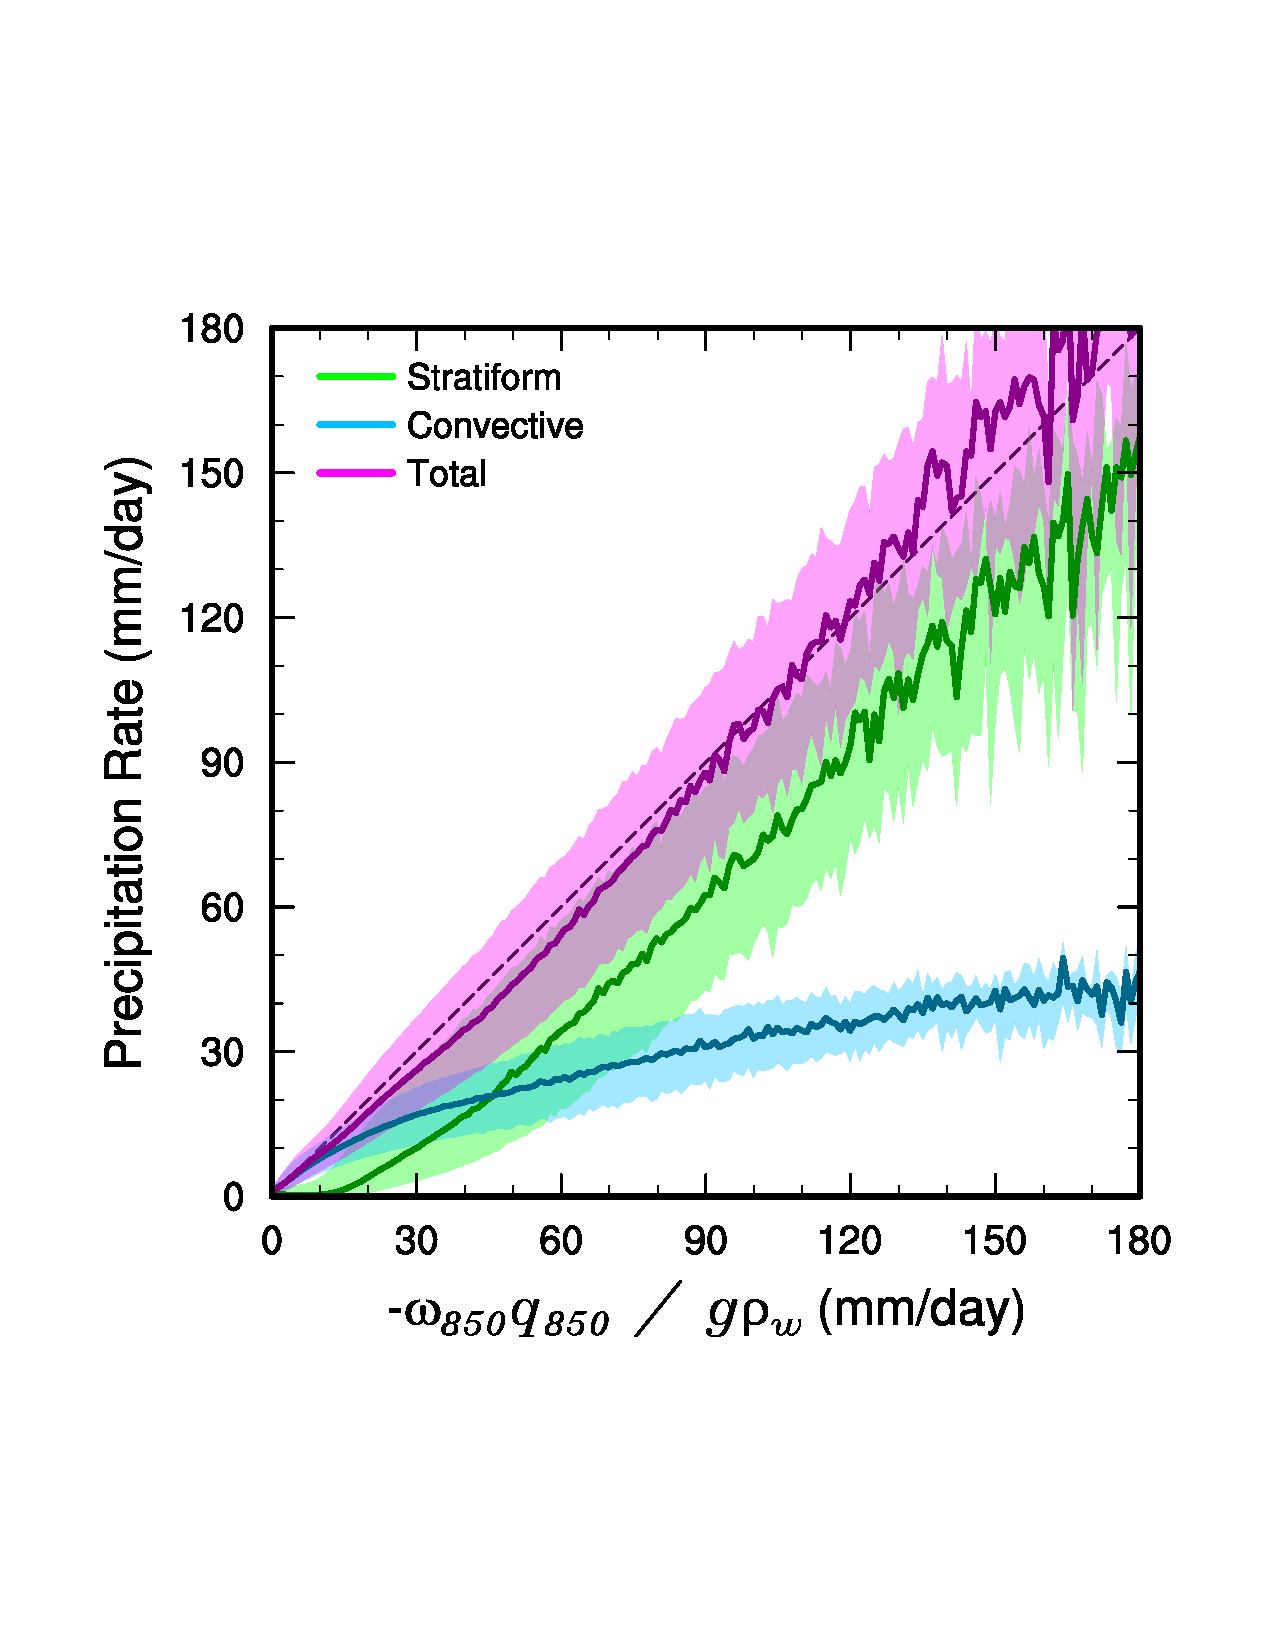
\includegraphics[width=20pc,angle=0]{figs/temp_mflux.pdf}\\
\end{center}
\caption{Precipitation rates vs. upward moisture flux at the 850 hPa level. Solid lines refer to median stratiform (green), convective (blue) and total (magenta) precipitation rates conditional on bins of the moisture flux, and shaded regions refer to the conditional interquartile ranges.}
\label{fig:mflux}
\end{figure}

To unravel the contributions of changes in $\omega$ and $q$ at the 850 hPa level $\omega_{850}$ and $q_{850}$, to the increase in global mean, climatological stratiform precipitation rates $\overline{P_s}$, $\overline{P_s}$ is decomposed in $\omega_{850}$ and $q_{850}$ space following \cite{TETAL2018CD}. Table~\ref{tbl:table2} indicates that the $\pm 15^{\circ}$ latitude band accounts for most of the change in global mean stratiform precipitation with resolution. The decomposition is then restricted to stratiform precipitation rates and moisture fluxes in the $\pm 15^{\circ}$ latitude region to simplify the analysis, and $\overline{P_s}$ is redefined as the average over $\pm 15^{\circ}$ latitude. 

$\overline{P_s}$ can be expressed as the double sum of the product of the time mean magnitude $M_s$ and time mean spatial frequency $f_s$, over $\omega_{850}$ and $q_{850}$ space,
\begin{equation}
\overline{P_{s}} = \sum_i \sum_j f_s \left( \omega_i , q_j \right) M_s \left( \omega_i , q_j \right) \label{eq:pdecomp}
\end{equation}
where the subscript $850$ is dropped from $\omega$ and $q$ for brevity. $f_s$ is a measure of the occurrence of a particular combination $\left( \omega_i , q_j \right)$ in a simulation, and $M_s$ the mean stratiform precipitation rate associated with the combination $\left( \omega_i , q_j \right)$. Their product $f_s M_s$ is then the contribution of a particular combination of $\left( \omega_i , q_j \right)$ to $\overline{P_s}$.

Figure~\ref{fig:pdecomp} shows plots of the terms $M_s$ and $f_s M_s$ for all resolutions. The plots are computed using 6-hourly instantaneous output of $\omega_{850}$ and $q_{850}$, with 0.05 Pa/s and 0.4 g/kg bin wdiths, respectively. Bins in  $\left( \omega_{i} , q_{j} \right)$ space with $f_s <1 \times 10^{-5}$ are masked out, which is a somewhat arbitrary, but still reasonable cut-off for a bins' contribution to $\overline{P_s}$. The $M_s$ plots (left column) show that larger magnitude $\omega_{850}$ correspond to larger magnitude stratiform precipitation rates, while the impact of changing $q_{850}$ on $M_s$ is less clear. The changes in $M_s$ with resolution are subtle, while the changes in $f_s$ with resolution are large (not shown). The changes to $f_s$ can be inferred from the larger space of $\left( \omega_i , q_j \right)$ plotted at higher resolutions, indicating that larger magnitude $\omega_{850}$ values are occurring more frequently at higher resolutions, above the cutoff for plotting. The $f_s M_s$ plots (right column) clearly shows that larger magnitude $\omega_{850}$, and therefore larger magnitude stratiform precipitation rates are contributing to the increase in $\overline{P_s}$ with resolution. In contrast, smaller magnitude $\omega_{850}$ and hence smaller stratiform precipitation rates contribute less and less to $\overline{P_s}$ with increasing resolution.

\begin{figure}
\begin{center}
\noindent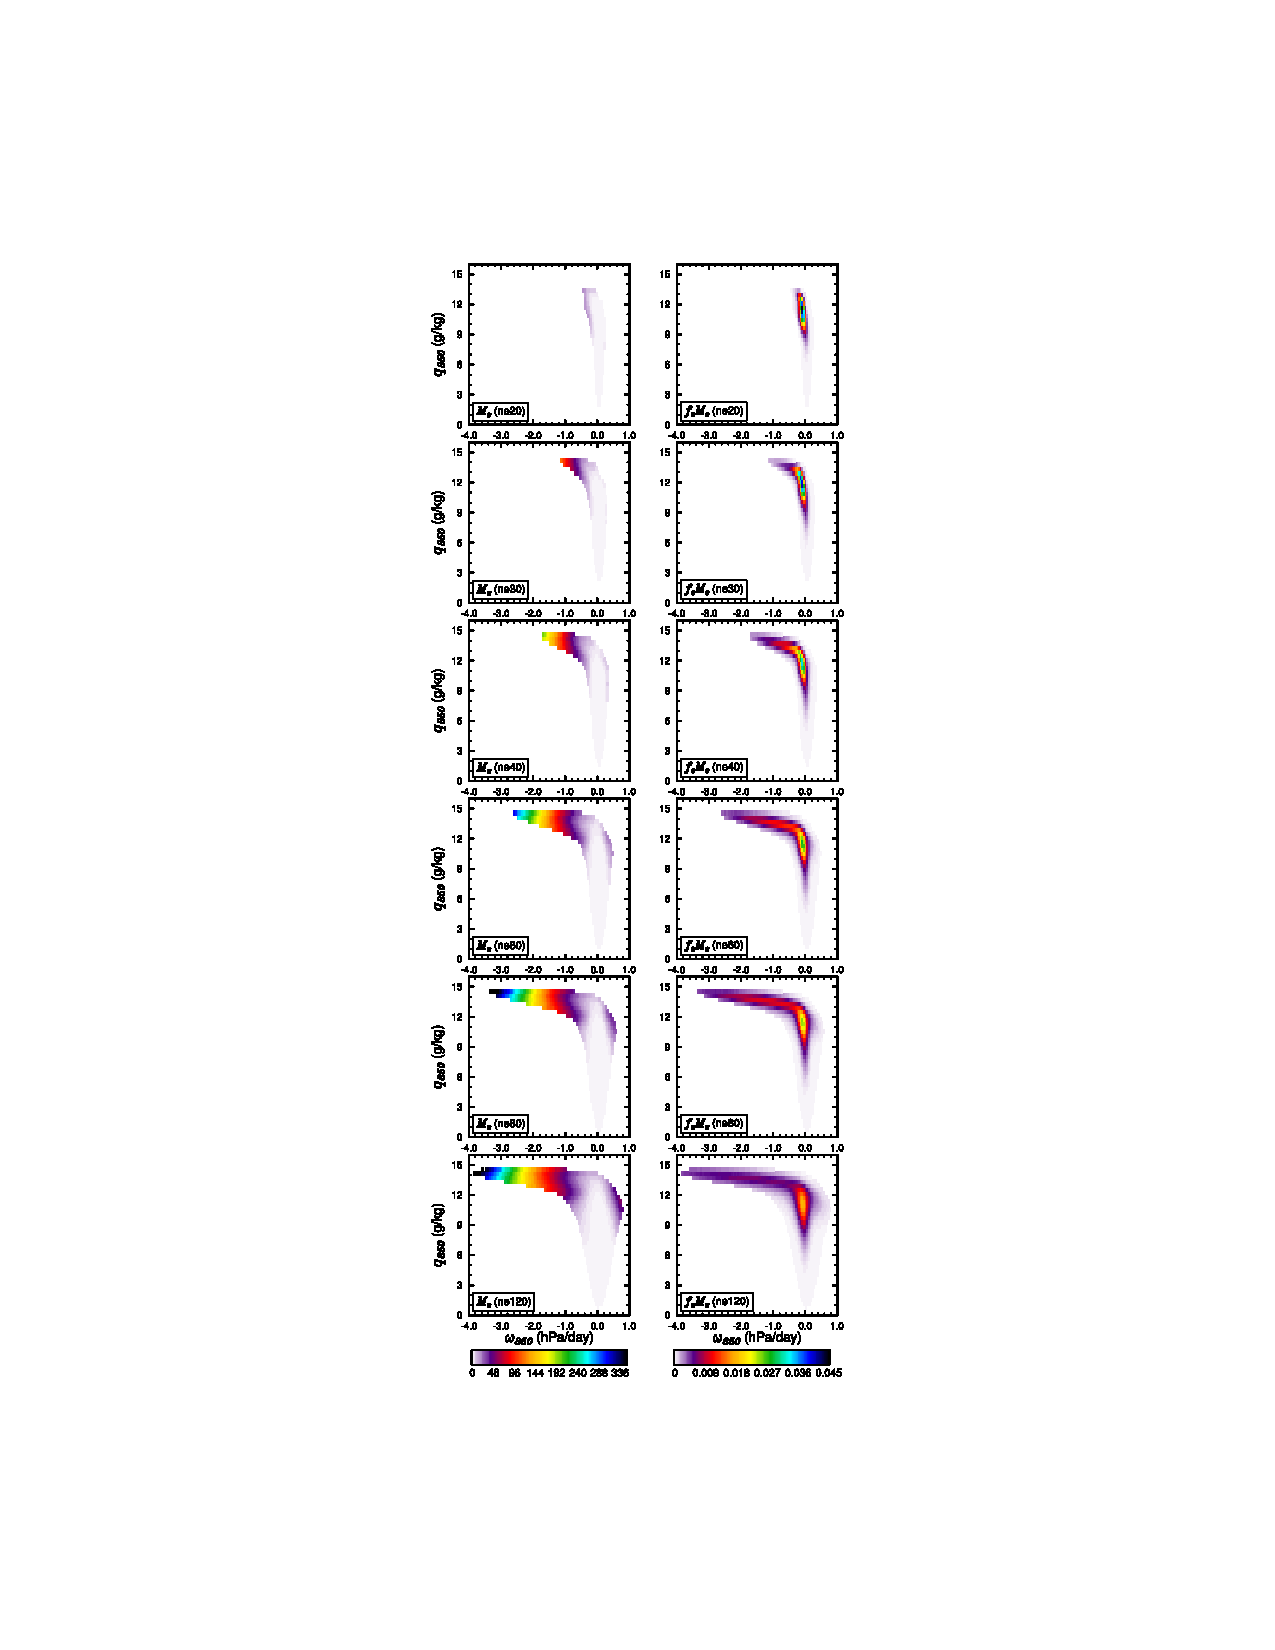
\includegraphics[width=20pc,angle=0]{figs/temp_pdecomp.pdf}\\
\end{center}
\caption{Decomposition of the climatological stratiform precipitation rates, averaged over the $\pm 15^{\circ}$ latitude band into $\omega_{850}$ and $q_{850}$ environmental conditions. Left column shows the time mean magnitude term $M\left( \omega_i , q_j \right)$ and the right column is the magnitude term multiplied by the space-time frequency term $f\left( \omega_i , q_j \right) M\left( \omega_i , q_j \right)$. Integrals over $f M$ gives the climatological, area averaged stratiform precipitation rate. Panel labels denote the grid resolution of the model run.}
\label{fig:pdecomp}
\end{figure}

\section{Conclusions}

Establishing a complete understanding of resolution sensitivity in atmospheric general circulation models (AGCMs) is crucial, since inevitable responses to native grid resolution cannot be ignored in the pursuit of scale-aware physics. This study analyzes a convergence experiment in an aqua-planet configuration using the Community Atmosphere Model (CAM), with the spectral-element dynamical core option coupled to the accelerated multi-tracer transport scheme (CAM-SE-CSLAM), and version 6 physics (CAM6), in order to understand longstanding convergence issues that have persisted within the CAM lineage since its inception (see Figure~\ref{fig:cam-history}). 

As with most versions of CAM, in CAM6 the atmosphere becomes drier and less cloudy with increasing resolution, and parameterized convective precipitation decreases while stratiform precipitation increases with resolution. Prior studies have established that the drying and reduction in cloudiness is a result of increases in the magnitude of vertical velocities with resolution, which more efficiently advect dry air aloft, downward \citep{KW1991JGR,WETAL1995CD,YETAL2014JCLIM,HR2017JCLIM}. This study aims to then understand why and how vertical velocities change with resolution, and why convective precipitation decreases at the expense of stratiform precipitation with increasing resolution.

The vertical velocities are found to fit a power law scaling $\Delta x^n$ with $\Delta x$ the grid spacing and $n=-1$. The $n=-1$ exponent is derived from a scale analysis of the Poisson equation, which shows pressure gradients scale like the inverse of the horizontal scale of buoyancy perturbations, $D^{-1}$, driving convergence into the air column and the vertical velocities also scale like $D^{-1}$. It has been previously shown that $D$ is set by stratiform cloud formation, which collapse to the smallest resolvable feature in the model \citep{HR2018JAMES}, the effective resolution \citep{S2011LNCSE}, and so $D \propto \Delta x$ and $n=-1$. This scaling is consistent with studies describing the resolution sensitivity of large-eddy simulations, which use similar physical arguments, but adapted for non-hydrostatic scales \citep{WETAL1997MWR,PG2006JAS,JR2016QJRMS}.

The $n=-1$ power law scaling is potentially in conflict with the scaling proposed by \cite{RETAL2016CD}, $n=h-1$, with $h$ being half the exponent of the second-order structure function $\Delta x^{2h}$ of the horizontal wind. \cite{RETAL2016CD} provide evidence for $h<1$ in their regional climate model simulations, and propose that $h=\frac{1}{3}$ is an emergent constraint for $n=-\frac{2}{3}$, based on observations. This is an intriguing proposal and the authors don't seek to dismiss its potential value. But it is suggested that the overwhelming support for the $h=\frac{1}{3}$ exponent in the second-order structure function is only relevant for horizontal scales on the order of $100$ km and less \citep{L1999JFM,CL2001JGR}, which is not resolved in even our highest resolution simulation $\Delta x=27.8$ km, since CAM-SE-CSLAM has an effective resolution in the range of $5-10\Delta x$ \citep{HETAL2019JAMES}. The nonexistence of $h=\frac{1}{3}$ in the $\Delta x=27.8$ km simulation is verified through analyzing the slope of kinetic energy spectrum $-\beta$, which is in duality with the second-order structure function through the Weiner–Khinchine theorem. For $h=\frac{1}{3}$, $\beta=\frac{5}{3}$, which is significantly less than the $\beta=3$ slope observed near the effective resolution in the simulation {\color{red}{(Figure~X)}}.

A strong negative correlation is discovered between the climatological, global mean activity of the \cite{ZM1995AO} deep convection scheme (ZM scheme) and global mean subsiding motion in the simulations. Since the ZM scheme is modulated by an entraining plume calculation, referred to as the dilute convective available potential energy (dilute CAPE), the authors sought to understand the influence of subsidence on dilute CAPE. In the deep tropics ($\pm 10^{\circ}$ latitude), subsiding regions have much smaller dilute CAPE values compared to ascending regions due to the influence of the drier, subsiding environment on dilute CAPE. With increasing resolution and in the deep tropics, the occurrence of subsiding motion increases dramatically and at the expense of ascending motion, and the activity of the the ZM scheme decreases overall. This is not completely unexpected due to the $\Delta x^{-1}$ scaling of the vertical velocities, e.g., a doubling of resolution can generate the same upward mass flux in just half the area. The increased efficiency of upward mass fluxes with resolution suggests that the occurrence of ascending motion can decrease with resolution while still maintaining statistical equilibrium with the large-scale forcing.

In addition to the change in balance of ascending/descending motion in the deep tropics, there is also a decrease in dilute CAPE of both ascending/descending regimes with increasing resolution. This reduction in background dilute CAPE is not confined to the deep tropics, but everywhere in the model and is in large part the reason for the global mean reduction in activity in the ZM scheme with resolution. A sensitivity analysis of the dilute CAPE calculation indicates that this change in background stability is primarily a result of temperature changes with resolution. The temperature changes reflect an increase in adiabatic warming due to increasing subsidence with resolution. 

Subsidence warming falls out of the component of the dilute CAPE budget due to the advection of dry static energy and moisture by the environment, commonly referred to as dynamic CAPE, or {\em{dCAPE}} \citep{XZ2000JGR,Z2002JGR}. Subsidence warming is represented in the dCAPE budget as negative the vertical advection of dry static energy, since warming the environment reduces dCAPE, and simplifies to $\frac{w}{c_{pd}} \frac{\partial gz}{\partial z} = \frac{g}{c_{pd}} w$, directly proportional to the vertical velocity $w$ by the factor $\frac{g}{c_{pd}}$, with $g$ the acceleration of gravity and $c_{pd}$ the specific heat capacity of dry air (F. Song, personal communication). The magnitude of negative, or downward $w$ increases everywhere in the model with increasing resolution, opposing the growth of dilute CAPE and reducing the activity of the ZM scheme with increasing resolution.

The subtropics ($\pm (10^{\circ}-30^{\circ})$ latitude) are uniquely less sensitive to subsiding motion. This is likely due to the the large, global maximum in surface latent heat fluxes in the subtropics, which increases dilute CAPE above the threshold for convection, but is restricted from growing too much larger due to substantial subsiding motion aloft. These opposing influences result in small values of dilute CAPE, and the ZM scheme acts more like a shallow convection scheme, producing copious amounts of light precipitation or drizzle, irrespective of resolution. 

AGCMs are known to suffer from an excess of drizzle relative to observations \citep{D2006JCLIM}. \cite{XETAL2019JAMES} recently proposed a new convective trigger for the ZM scheme that the authors suggest may alleviate the excess drizzle bias in CAM. As with the ZM scheme used in this study, dilute CAPE must exceed a threshold for convection to occur, but \cite{XETAL2019JAMES} also require dCAPE to be positive. Based on the analysis in this study, and the strong connection between vertical velocities and dCAPE reported in \cite{SZ2018JCLIM}, it is reasonable to speculate that dCAPE is often negative in drizzling regions, which may prevent the ZM scheme from triggering. The authors suggest that the \cite{XETAL2019JAMES} trigger be explored as a means to mitigate the drizzling bias in CAM.

The stratiform scheme becomes more active with resolution, compensating for the reduction in activity of the ZM scheme with resolution, particularly as it relates to the Intertropical Convergence Zone (ITCZ). Energetically, it is expected that stratiform precipitation rates increase with resolution to compensate for the reduction in convection from the ZM scheme in order to balance radiative cooling. But this argument requires one to assume the increase in stratiform precipitation is responding to a reduction in ZM activity, whereas this study indicates the reverse, that the ZM scheme is responding to increases in subsidence with resolution, driven by greater ascent associated with stratiform cloud formation. The authors instead sought to understand the increase in stratiform precipitation with resolution at the process level. It is shown that resolved upward moisture fluxes are highly correlated with stratiform precipitation rates, and that there is an increase in both upward moisture fluxes and stratiform precipitation with resolution. Through decomposing the stratiform precipitation in the ITCZ region into the components of the moisture flux, it is shown that larger magnitude vertical velocities are associated with larger stratiform precipitation rates, and these large precipitation rates increasingly contribute to the increase in climatological stratiform precipitation rate with resolution.

{\color{red}{Wrap up with a closing paragraph}}

\ack 
Funding support for this work was in part provided by the U.S. Department of Energy Office of Science (DE-SC0019459) and the National Science Foundation (AGS1648629 and AGS1830729). Computing and data storage resources, including the Cheyenne supercomputer (doi:10.5065/D6RX99HX), were provided by the Computational and Information Systems Laboratory (CISL) at the National Center for Atmospheric Research (NCAR). Herrington would like to thank Dr. Sultan Hameed for his assistance with the statistical analysis used in this study.

\bibliographystyle{wileyqj}
\bibliography{bib}
\end{document}
